\documentclass[11pt]{article}

% ---------- Packages ----------
\usepackage[margin=1in]{geometry}
\usepackage{setspace}
\onehalfspacing
\usepackage{amsmath,amssymb,amsfonts,amsthm}
\usepackage{mathtools}
\usepackage{bm}
\usepackage{enumitem}
\usepackage{booktabs}
\usepackage{graphicx}
\usepackage{xcolor}
\usepackage{comment}
\usepackage{algorithm,algpseudocode}
\usepackage{natbib}
\setcitestyle{round,semicolon}
\usepackage{float}    % enables [H] placement
\usepackage{placeins} % enables \FloatBarrier
\usepackage{xurl}
\usepackage{hyperref}
\hypersetup{
  pdftitle={Designing Customer Feedback for Subscription Curation},
  pdfauthor={Renjun Hu, Hyun-Soo Ahn, Stefanus Jasin},
  pdfkeywords={subscription curation, customer feedback, Bayesian learning, value of information, top-K selection}
}
\hypersetup{
  colorlinks=true,
  linkcolor=blue!60!black,
  citecolor=blue!60!black,
  urlcolor=blue!60!black
}
\Urlmuskip=0mu plus 1mu\relax

% ---------- Theorem-like environments ----------
\newtheorem{theorem}{Theorem}
\newtheorem{proposition}[theorem]{Proposition}
\newtheorem{lemma}[theorem]{Lemma}
\newtheorem{corollary}[theorem]{Corollary}
\theoremstyle{definition}
\newtheorem{definition}{Definition}
\newtheorem{condition}{Condition}
\theoremstyle{remark}
\newtheorem{remark}{Remark}

% ---------- Macros ----------
\newcommand{\R}{\mathbb{R}}
\newcommand{\V}{\mathcal{V}}
\newcommand{\E}{\mathbb{E}}
\newcommand{\Var}{\mathbb{V}\mathrm{ar}}
\newcommand{\Prob}{\mathbb{P}}
\newcommand{\1}{\mathbf{1}}
\newcommand{\w}{\mathbf{w}}
\newcommand{\norm}[1]{\left\lVert #1\right\rVert}
\newcommand{\abs}[1]{\left\lvert #1\right\rvert}
\newcommand{\trace}{\mathrm{tr}}
\newcommand{\diag}{\mathrm{diag}}
\newcommand{\lammin}{\lambda_{\min}}
\newcommand{\lammax}{\lambda_{\max}}
\newcommand{\Normal}{\mathcal{N}}
\newcommand{\bmu}{\boldsymbol{\mu}}
\newcommand{\bkappa}{\boldsymbol{\kappa}}
\newcommand{\bSigma}{\boldsymbol{\Sigma}}
\newcommand{\N}{\mathbf{N}}
\newcommand{\bS}{\mathbf{S}}
\newcommand{\Ceq}{\mathcal{C}}
\newcommand{\p}{\mathbf{p}}
\newcommand{\cN}{\mathcal{N}}
\newcommand{\cD}{\mathcal{D}}
\newcommand{\Cov}{\text{Cov}}
\newcommand{\bA}{\mathbf{A}}
\newcommand{\cO}{\mathcal{O}}
\newcommand{\bH}{\mathbf{H}}
\newcommand{\cF}{\mathcal{F}}
\newcommand{\bu}{\mathbf{u}}
\newcommand{\bt}{\mathbf{t}}
\newcommand{\cR}{\mathcal{R}}


% Problem-specific shorthand
\newcommand{\VK}[1]{V_K\!\left(#1\right)}          % Ky Fan top-K
\newcommand{\TopK}{B^\star}                        % true top-K set
\newcommand{\Loss}{\Delta}                         % next-box value gap
\newcommand{\SigPrior}{\bSigma}                   % prior covariance
\newcommand{\MuPrior}{\mu}                         % prior mean vector
\newcommand{\Info}{\mathcal{I}}                    % Fisher information
\newcommand{\SigPost}{\Sigma_N}                    % posterior/asymptotic covariance
\newcommand{\e}{\mathrm{e}}

% ---------- Title ----------
\title{\vspace{-1em}\textbf{Designing Customer Feedback for Subscription Curation}}
\author{
Renjun Hu \qquad Hyun-Soo Ahn \qquad Stefanus Jasin \\[0.6em]
Ross School of Business, University of Michigan \\[0.25em]
\small \texttt{renjunhu@umich.edu} \qquad \texttt{hsahn@umich.edu} \qquad \texttt{sjasin@umich.edu}
}
\date{August 2026}

\begin{document}
\maketitle

% ---------- Abstract ----------
\begin{abstract}
Subscription services that curate on the customer's behalf, such as a
meal-kit service choosing next week's recipes, must decide what to ship
before knowing what each customer likes. The costly mistake is to ship
a product the customer values less while a better one stays behind. In
an industrial curation log analyzed by one of the authors, the
composition of shipped boxes is associated with customer retention.
Customer feedback could prevent such mistakes, but it is scarce.
Richer questionnaires teach more per answer while fewer customers
complete them.

We study the two feedback decisions the platform makes before each
shipment. The first is the format. How many questions should a
questionnaire have, and how rich a rating scale? We introduce Effective
Information Supply (EIS), the expected usable information per customer
shown the questionnaire. When a change of rating scale multiplies the
information of every product by the same factor, ranking formats by EIS
is exactly optimal; otherwise it is a practical first screen. The
second is targeting. A Bayesian analysis shows that losses concentrate
on products near the boundary between shipping and not shipping, where
a small estimation error changes what ships.

Calibrated with public data, EIS shows that the best format depends on
the response environment. Under survey-like completion loss a richer
five-point format wins; under the steeper loss observed in Netflix's
in-product test, simple binary prompts win. For targeting, a simple guarded rule performs best in the synthetic
tests. It asks about products near the shipping boundary and asks less
about products that already have many answers. Rules that target
uncertainty alone can lose even to spreading questions evenly. In chronological MovieLens ratings, boundary-focused rules beat uniform
sampling and recover roughly \(15\) to \(40\) percent of the lost
shipment value.
\end{abstract}

% =========================================================
\section{Introduction}

A curation subscription does more than refill a product the customer
already knows. It sends a recurring box whose contents the retailer
chooses. The global subscription-box market was valued at about \$30
billion in 2024. Forecasts expect continued growth
\citep{ResearchAndMarkets2025}.
Curation services now appear in meal kits, online groceries, beauty, and
apparel. Customers pay for convenience, discovery, and personal fit.
Getting them to subscribe is only the first step. Because the model earns
revenue over time, retention is a core business metric. Each new box must
still feel worth it. A box that feels random, repetitive, or poorly
matched gives the customer less reason to stay \citep{ChenEtAl2018}.
Product choice is therefore more than a fulfillment decision. Each box
can strengthen or weaken the customer's reason to continue.

Feedback can make the next box better. Ratings from one cycle can guide
the next. Stitch Fix and Hungryroot, for example, tell customers that
current ratings and preferences shape future deliveries
\citep{StitchFixBestFix2025,HungryrootPersonalized2025,HungryrootPreferences2025}.
But asking for feedback is not free. Every extra question takes time and
adds friction. A longer survey may collect more ratings from each person
who finishes it. It may also lead more people to quit. Many surveys get
responses from only 10 to 30 percent of customers. Online surveys average
about 29\%, while in-app surveys average about 13\% \citep{Malnik2025}.
The retailer must therefore make two choices before the next deadline.
What kind of feedback should it request? Which products should it ask
about?

More answers alone do not solve this problem. Better predictions across
the whole catalog may not solve it either. Consider a meal-kit service
that must choose five recipes from forty. Better estimates for the most
and least popular recipes may not change the menu. The difficult choice
is between recipes around fifth place. The retailer may leave out a
better recipe and ship a weaker one. We call this a \emph{wrong swap}.
Feedback is useful when it can prevent that swap before the menu is
locked.

The cutoff also shows where the next question may help most. A product
near the cutoff is worth asking about if one more rating could change
whether it ships. One rating may also teach the retailer about other
products. This can happen when items share a brand, category, style,
cuisine, or use. The best next question is the one most likely to improve
the box. Its value may come from the product itself or from what it
reveals about similar products.

Our paper studies these two choices. A feedback plan is better when it
leads to a better next box. We call the value lost from imperfect
feedback the \emph{next-box value gap}. The retailer first chooses how
to ask for feedback. We introduce Effective Information Supply (EIS) to
compare these formats. EIS combines survey length, how many customers
finish, and how much each answer teaches. The retailer then decides which
products should receive the questions. The first choice controls how much
useful information arrives. The second decides where to use it.

\paragraph{Contributions.}
Our analysis makes three contributions.
\begin{enumerate}[leftmargin=*]
\item \textbf{We introduce Effective Information Supply (EIS) to compare
feedback formats.}
EIS measures the useful information produced for each customer who sees
the survey. It reflects three things. How many questions does the survey
ask? How many customers finish it? How much does each answer teach? We show when these three numbers are enough to choose a format. The key
condition asks that a change in rating scale change the information from
every product by the same proportion. Under this condition, the
format with the highest EIS also gives the highest expected value for
the next box. When the condition is only approximate, EIS provides a
first screen.

\item \textbf{We show where customer feedback has the most value.}
We show why feedback should focus on the shipment cutoff. Our main result
links the value of asking about a product to two things. How much is
still unknown about the product? How likely is it to sit at the cutoff?
Products that are clearly in or out of the box receive little attention.
The resulting rule focuses on products near the cutoff and moves on as
ratings arrive.

\item \textbf{We test the design rules in simulations and with MovieLens
ratings.}
In our main simulations, the guarded cutoff rule performs best. It asks
about products near the cutoff, then moves on as ratings arrive. More
detailed estimates help mainly when the budget is tight. They also help
when the products near the cutoff have very different numbers of past
ratings. We estimate the inputs to EIS from MovieLens ratings, published
response rates, and a randomized study of survey length. We also test
the allocation rules on MovieLens ratings in time order. The same broad
pattern appears.
\end{enumerate}

The remainder of the paper proceeds as follows. Section~2 reviews related
work. Section~3 defines the curation problem and the next-box value gap.
Section~4 explains why feedback matters most near the shipment cutoff.
Section~5 compares feedback formats with EIS. Section~6 shows how to
allocate the answers that arrive. Section~7 reports the numerical
experiments. The Appendix contains proofs and supporting analyses.

\section{Related Literature}
\label{sec:lit}

The work closest to ours allocates a measurement budget to select the
best few alternatives, in ranking and selection and in dynamic
assortment. We engage it directly in the second part of this review.
The broad difference is the information source. Those procedures draw
replications from a simulator or observe sales on a shelf. A curation
platform must collect short answers from busy customers, so the design
of the questionnaire decides how much information exists at all. The
review has three parts. The first covers how platforms learn from short
ordinal signals and what asking costs the customer. The second covers
how to value learning by the decision it changes. The third covers
how beliefs about related products connect.

\subsection{Ordinal elicitation, survey burden, and feedback format design}

Ordinal-response models let platforms learn from short, easy signals such
as likes, ratings, comparisons, and rankings, and a long statistical
literature shows how such signals identify preferences
\citep{BradleyTerry,Plackett,Luce,McCullagh,Agresti,Hunter,CaronDoucet,GuiverSnelson}.
Tools for ranking consistency, Gaussian-process ordinal regression,
and one-bit or implicit feedback extend this learning to sparse
customer signals
\citep{NegahbanOhShah2012,MaystreGrossglauser2015,ChuGhahramani2005,Joachims2002,HuKorenVolinsky2008}.
In marketing, adaptive conjoint designs tailor later questions to
earlier answers so that preferences are learned efficiently
\citep{ToubiaHauserSimester2004,ToubiaHauserGarcia2007,YuGoosVandebroek2011,SaureVielma2019}.
Customer engagement research adds the behavioral side. Ratings and
reviews are voluntary contributions, offered when the interaction is
worth the customer's effort
\citep{VerhoefReinartzKrafft2010,VanDoornEtAl2010,PansariKumar2017}.

Our setting adds the format itself to the operating decision. The
platform chooses an instrument whose length and response scale affect
how many customers answer before the deadline and how much each
completed answer carries. Survey research documents both effects.
Longer or more demanding instruments reduce participation and can
change response quality
\citep{Krosnick1991,Galesic2009,Rolstad2011,Peytchev2009,FanYan2010,DillmanSmythChristian2014,Callegaro2015},
and asking more elicitation questions can reduce external validity as
respondents adapt to the task
\citep{HowellEbbesLiechty2021,LiEtAl2022MoreYouAsk}. The literature
measures these costs. EIS prices them into a single score a platform
can act on.

\subsection[Value of information and top-K decisions]{Decision-focused learning, value of information, and top-$K$ decisions}

The decision-focused side of the paper builds on work that values
learning by what it changes downstream. Pure exploration and best-subset identification ask how to find the best
arms or the right top-$K$ set
\citep{KalyanakrishnanEtAl,KaufmannEtAl,GabillonEtAl,ChenEtAlCPE,KalyanakrishnanTewari,KomiyamaEtAl,KvetonEtAl}. The objective is identification, and cumulative reward plays no role.
Bayesian value-of-information, knowledge-gradient, and optimal-design
methods judge a measurement by its decision value
\citep{FrazierPowellDayanik,RussoVanRoy,ChalonerVerdinelli1995,AtkinsonDonevTobias2007,SandorWedel2001,KesselsGoosVandebroek2006,BliemerRose2011,ElmachtoubGrigas2022}.
Our marginal value of additional responses is a rule of exactly this kind.

The closest operations work allocates a measurement budget to select
top alternatives. Optimal computing budget allocation (OCBA) decides
how many simulation replications each alternative receives, including subset-selection variants that target the best \(m\) alternatives at once \citep{ChenLinYucesanChick2000,ChickInoue2001,ChenHeFuLee2008}.
Dynamic assortment models with demand learning balance the same
exploration trade-off across retail products
\citep{CaroGallien2007,SaureZeevi2013}. Our allocation step shares the
top-\(K\) structure of this work, and the lesson that scarce
measurements belong near the selection boundary echoes those
procedures. Two features still separate the feedback-design problem.
In that literature the information source is a simulator. Here it is a
customer, so how much information arrives is itself a design lever, and
Section~\ref{sec:feedback_design} prices that lever before any
allocation. And the signals are ordinal ratings whose information content depends on
the chosen response scale, while the replication literature draws from a
homogeneous noise channel. The outputs differ as well. OCBA-style
procedures produce asymptotically optimal replication ratios. Ours is a
priority score for a recurring curation cycle, and
Section~\ref{subsec:design-allocation} compares the two directly.

A different tradition, active learning, ranks queries by how uncertain
the model is about them \citep{Settles2009}. Our experiments include
that rule as a baseline, and it performs poorly, because uncertainty
has decision value only where resolving it can still change the box.
Section~\ref{sec:gap-analysis} makes that statement exact.

\subsection{Correlated priors and spillover learning}

Product feedback is rarely isolated. A response about one item can
sharpen beliefs about related items that share a brand, category,
style, cuisine, or usage occasion. Gaussian-process priors carry this
idea through Bayesian optimization and bandits
\citep{SrinivasEtAl,ContalEtAl,DesautelsEtAl,ValkoEtAl,KrauseGuestrin,Seeger}.
Gaussian Markov random fields and related graph models make the same
structure tractable at scale \citep{KondorLafferty,RueHeld,Lauritzen}.
Classical experimental design studies it under criteria such as
entropy, mutual information, and estimation precision
\citep{Pukelsheim}. From this line we borrow only the machinery, a
correlated Gaussian prior with conjugate updating.

Our use of correlation is narrower and tied to the shipment decision.
Correlation matters when it changes which products deserve direct
questions before the next box is fixed. If one answer also reduces
uncertainty for several near-cutoff alternatives, that answer can be
worth more than a direct question about an isolated product. Our
allocation rule prices exactly that possibility.

\section{Problem Setting}\label{sec:problem-setting}

This section builds the model in four steps, each organized around a
question the platform faces. What must be decided before the deadline?
What is unknown when that decision is made? What can be observed before
the box is locked? And how should the platform measure whether feedback
was worth collecting? The meal-kit example from the introduction runs through the section, and
each formal object is introduced where its question arises.

\subsection{The curation decision}\label{subsec:biz-data}

Return to the meal-kit service from the introduction. Its forty
candidate recipes might be the vegetarian menu, curated separately from
the rest of the catalog. We call such a decision unit a \emph{curation
segment}. One segment might be the vegetarian menu, another the family
plan, another a style profile at an apparel service. The platform has
already narrowed the feasible catalog for the segment, and it chooses
\(K=5\) recipes from these \(L=40\) before the next menu is locked. The
final shipment can still be personalized downstream. The segment is the
unit at which the platform decides what feedback to ask for and how to
use the answers.

Let $\mathcal I := \{1,\dots,L\}$ denote the candidate catalog for the
segment. In each period $t$, a customer receives a box
$B_t \subseteq \mathcal I$ containing $K$ items, with \(1\le K<L\), so
the box is a strict selection from the catalog. Receiving item
$i \in B_t$ generates a latent utility $u_{it}$ for customer $t$, and
we take the customer's total utility from the box to be additive,
\[
U_t(B_t) \;:=\; \sum_{i \in B_t} u_{it}.
\]
Additivity is a deliberate simplification with a clear division of
labor. Inventory, variety, repetition, and complementarity constraints
are handled upstream, when the feasible catalog for the segment is
constructed. Conditional on that catalog, the remaining question is
which items the segment values most. Box value is then the sum of the
items' values. Expected box value is the quantity the platform tries to
improve when it collects feedback before the next shipment.

\subsection{What the platform does not know}\label{subsec:unknown}

If the platform knew how much the segment valued each candidate item,
the problem would be easy. The platform would ship the \(K\) most valued
items. The unknown
is the persistent part of item value. We separate it from
customer-level idiosyncrasy by writing
\[
u_{it} \;=\; w_i + \varepsilon_{it},
\qquad \varepsilon_{it} \overset{\text{i.i.d.}}{\sim} \mathcal N(0,1),
\]
independently across items $i$ and customers $t$ within the segment.
In the meal-kit example, $w_i$ is the average appeal of recipe $i$
among the segment's customers, and \(\varepsilon_{it}\) captures how an
individual customer's reaction deviates from that average.

This separation fixes the learning target. The model estimates the
segment-average values collected in the vector \(\mathbf w\). These
values determine which candidates belong in the segment's box;
customer-level tastes can still be handled by downstream
personalization. Because the target is shared across
customers, every answer from any customer in the segment is informative
about the same vector \(\mathbf w\). This pooling is what makes
learning from sparse feedback feasible.

The platform starts from a Gaussian prior,
\[
\mathbf w \sim \mathcal N(\bmu,\ \bSigma),
\]
with mean vector $\bmu \in \mathbb R^L$ and positive-definite
covariance matrix $\bSigma \in \mathbb R^{L \times L}$. The prior mean
records what the platform already believes about each item.
Correlations in $\bSigma$ encode menu knowledge. Two similar curry
recipes tend to be valued similarly, and so do items that share a
brand, cuisine, or flavor, or that sit close in a metadata or
co-preference embedding. Learning about one such item teaches the
platform about the other.

\subsection{What the platform can observe}\label{subsec:estimator}

Customers do not report utilities. They tap short prompts, such as a like or dislike, a star rating, or another small set of ordered satisfaction
categories. Let \(S\) denote the number of ordered response categories
and \(\cR_S=\{1,\ldots,S\}\) the rating set, so a like/dislike prompt
has \(S=2\), a like/neutral/dislike system has \(S=3\), and a
five-star rating has \(S=5\). Based on realized utility \(u_{it}\),
customer \(t\) reports a rating \(R_{it}\in\cR_S\) according to an
ordered-probit model with thresholds
\[
-\infty = \theta_0 < \theta_1 < \cdots < \theta_S = +\infty,
\]
so that\footnote{Other ordered-response
models, such as ordered logit, lead to the same managerial trade-offs.
We use the probit form for concreteness.}
\[
\Pr(R_{it} = s \mid w_i)
\;=\;
\Phi(\theta_s - w_i) - \Phi(\theta_{s-1} - w_i),
\qquad s \in \cR_S.
\]

Responses can arrive through two routes. In post-consumption rating, a
customer who received item \(i\) in an earlier box reacts to the
realized experience \(u_{it}\), as written above. The platform can also ask before shipping. It shows a candidate item and
requests a quick reaction. We model such pre-shipment preference prompts through the
same ordinal channel. The noise term then also absorbs the extra
imprecision of judging an item that has not yet been consumed. We study active feedback designs, in which the platform chooses which
items to ask about. Pre-shipment prompts satisfy this directly. Post-
consumption ratings satisfy it for items the platform can still expose.
Historical ratings arrive only for items that earlier boxes shipped, and
correcting that exposure bias lies outside the present analysis. Within
an active design, two quantities matter for the next-box decision, how
many answers arrive and how much each answer teaches about \(\mathbf
w\).

The first quantity is the response budget. Customer attention is
scarce, so once a questionnaire format is chosen, the platform records \(N_i\) submitted responses on item \(i\), and the total is expected to stay within a budget,
\[
\sum_{i=1}^L N_i \le N_{\text{tot}}.
\]
The second quantity is how much one completed answer teaches, which we
summarize with the standard Fisher-information measure. Let
\(I_S(w_i)\) denote the information in one ordinal response about item
\(i\) under scale \(S\), and define the scale-specific average
information in one answer as
\[
\kappa_i(S) \;:=\; \E_{w_i}\!\big[I_S(w_i)\big].
\]
Readers can interpret \(\kappa_i(S)\) as how much one completed rating
teaches about product \(i\) under scale \(S\); for a fixed chosen
format we write \(\kappa_i\). Coarser feedback typically lowers
information per completed answer, while finer scales can raise it if
customers complete the task. Section~\ref{sec:feedback_design} returns
to this trade-off between completion and per-answer information by
normalizing average \(\kappa_i(S)\) relative to a baseline scale.

As answers accumulate, beliefs sharpen in an intuitive way. An item
with few recorded answers is judged mostly by what the prior says about
it; an item with many answers is judged mainly by its data. Because
\(\bSigma\) links related items, an answer about one curry recipe also
sharpens the platform's view of similar recipes. The next subsection
turns these beliefs into a decision and into a measure of decision
quality.

\subsection[Measuring value loss]{Measuring the value loss from imperfect feedback}\label{subsec:retention}

After the feedback window closes, the platform holds data
\(\mathcal D\) and must commit to a box. It forms the posterior-mean
estimate of the segment values,
\begin{equation}\label{eq:postmean-def}
\hat{\mathbf w}
\;:=\; \mathbb E\!\big[\mathbf w \,\big|\, \mathcal D\big],
\end{equation}
and ships the \(K\) items with the highest estimated values. We call
this estimate-based rule the plug-in top-\(K\) policy. The natural
benchmark is an oracle that knows the true vector \(\mathbf w\) before
choosing the box. Formally,
\[
B^*(\w) \in
\arg\max_{\substack{B\subseteq\{1,\ldots,L\}\\ |B|=K}}
\sum_{i\in B} w_i,
\qquad
\hat B(\hat{\w}) \in
\arg\max_{\substack{B\subseteq\{1,\ldots,L\}\\ |B|=K}}
\sum_{i\in B} \hat w_i,
\]
with ties resolved by any fixed rule. The first is the box an
all-knowing curator would ship; the second is the box the platform
actually ships after learning from sparse feedback.

We evaluate feedback by how much shipped value this difference costs.
The next-box value gap from the introduction now has a formal
definition,
\begin{equation}\label{eq:def-delta}
\Delta_{\mathrm{ord}}
:=
\underbrace{\mathbb E_{\w}\!\Big[\sum_{i\in B^*(\w)} w_i\Big]}_{\text{oracle top-$K$ value}}
-
\underbrace{\mathbb E_{\w,\mathcal D}\!\Big[\sum_{i\in \hat B(\hat{\w})} w_i\Big]}_{\text{plug-in value}}
\;\;\ge\;0.
\end{equation}
The gap carries the paper's retention motivation. Boxes that miss what
customers value give them less reason to continue, and an observational
analysis of an industrial subscription curation log supports this link.
A one-standard-deviation rise in repeated items is associated with
twelve to thirty-seven percent lower odds of retention, depending on
the segment; larger boxes are associated with higher retention, and
heavier premium intensity with lower retention
(Appendix~\ref{app:retention-drivers}). Some of these levers sit upstream of our weight model, in the catalog
construction. The evidence supports a narrower point. Retention moves
with what ships in the box. We use that association as motivation, and
the estimates remain observational.

\(\Delta_{\mathrm{ord}}\) measures the shortfall in shipped value that better feedback could have prevented. Better feedback keeps a better item in the box instead of a weaker substitute. The gap is therefore the objective against which feedback formats and allocations are compared in the rest of the paper.

For later use, define the top-$K$ value functional
\(V_K(\mathbf x) := \sum_{r=1}^{K} x_{(r)}\), where
$x_{(1)} \ge \cdots \ge x_{(L)}$ denote the order statistics of
$\mathbf x$, so that $V_K(\w)=\sum_{i\in B^*(\w)} w_i$. Because the
posterior mean is the platform's forecast of the true item values, the
plug-in value equals the expected top-\(K\) value of \(\hat{\mathbf w}\)
(Appendix Lemma~\ref{lem:posterior-value}). The gap therefore has the
compact form
\begin{equation}\label{eq:delta-VK}
\Delta_{\mathrm{ord}} \;=\; \E\!\big[V_K(\w)\big]\;-\;\E\!\big[V_K(\hat{\w})\big].
\end{equation}
When the feedback allocation is explicit, we write the same
ordinal-feedback gap as \(\Delta_{\mathrm{ord}}(\N)\).

\paragraph{Multiple curation segments.}\label{subsec:finite-segments}
The notation above suppresses segment indexes, which keeps attention on
one next-box decision. Many platforms operate several curation segments
at once. If each segment has its own feedback format and its own
response budget, the problem separates, and the analysis applies
segment by segment. When segments share a format or a common pool of
responses, the allocation unit becomes a segment-item pair. A segment's
claim on the next question then depends on two things, its decision
weight and whether another answer can still change its own box. A
large segment with a settled decision can be lower priority than a
smaller segment with a contested one.
Section~\ref{sec:alloc_opt} makes this priority operational, and
Appendix Proposition~\ref{prop:finite-segments} gives the formal
statement.

\paragraph{One number and two levers.}
The rest of the paper is organized around the single number defined
above, the value lost in the next box, and the two design levers that
shrink it. Section~\ref{sec:gap-analysis} shows which items carry the loss. It
splits item by item into remaining uncertainty times the chance of
sitting at the shipment cutoff. Section~\ref{sec:feedback_design} sets
the format lever and Section~\ref{sec:alloc_opt} the allocation lever.
Section~\ref{sec:numerics} tests both.

\section{Why the Shipment Cutoff Drives Feedback Value}
\label{sec:gap-analysis}

After the decision rule is fixed, the platform needs to know which
uncertainty is worth reducing before the next box ships. Precision
matters most when it can change membership around the top-\(K\) cutoff.
We first introduce a Gaussian proxy that summarizes how much uncertainty
the planned feedback resolves and how much remains. We then show that
the remaining decision errors concentrate at the shipment cutoff, the
line between the last item shipped and the first item left out. This
yields an explicit formula for the value lost and, in
Section~\ref{sec:alloc_opt}, a way to rank the next response.

\subsection{A Gaussian proxy for what feedback resolves}
\label{subsec:proxy}

To say where decision loss lives, we first need to describe what
remains unknown after the planned feedback has been collected. The
ordered-probit model of Section~\ref{subsec:estimator} remains the
behavioral model for ratings. To obtain tractable formulas, we work with a
\emph{Gaussian information proxy}. The proxy keeps the same belief-updating structure and returns a compact
summary of that residual uncertainty. In the proxy, each recorded answer about item \(i\) is treated as a
Gaussian signal about \(w_i\) carrying the same average information
\(\kappa_i\) as one ordinal response. Standard Gaussian updating then gives the residual covariance of \(\w\) after allocation \(\N\),
\[
A(\N):=\big(\bSigma^{-1}+\operatorname{diag}(N_i\kappa_i)\big)^{-1}.
\]
Small entries of \(A(\N)\) mean that little uncertainty about the
corresponding items remains once the answers are in.

The proxy also describes the platform's position before the answers
arrive. This matters because the format and the allocation must be
chosen at that point. Before the answers come in, the platform cannot
know what they will say. So it cannot know where its estimate will
land. Informative answers would move the estimate far from the prior
mean. Uninformative answers would leave it close by. Prior uncertainty
thus splits into two parts. The part the planned feedback will resolve
shows up as movement of the estimate. The part that will remain is
\(A(\N)\). The proxy posterior mean accordingly has distribution
\[
\tilde{\w}(\N) \sim
\mathcal N\!\big(\bmu,\ \bSigma - A(\N)\big).
\]
The two extremes clarify the interpretation. With no feedback,
\(A(0)=\bSigma\), so \(\tilde{\w}(0)\) is degenerate at \(\bmu\) and
the platform ranks products by prior means alone. As feedback becomes
precise, \(A(\N)\) shrinks toward zero and \(\tilde{\w}(\N)\)
approaches the distribution of the true vector \(\w\). Feedback moves
the platform from prior-mean curation toward fully informed curation.

When we derive explicit formulas, we use the Gaussian-proxy decision
gap
\begin{equation}\label{eq:delta-proxy}
\Delta(\N)
:=
\E\!\big[V_K(\w)\big]-\E\!\big[V_K(\tilde{\w}(\N))\big],
\end{equation}
the proxy analogue of the next-box value gap \eqref{eq:delta-VK}. From
this point forward, \(\Delta(\N)\) denotes the proxy gap unless we
explicitly refer to the ordinal-feedback gap \(\Delta_{\mathrm{ord}}\).
The proxy translates sparse ordinal reactions into uncertainty over
contested products. That is the uncertainty that can still change the
next box. With \(\Delta(\N)\) in hand, the next two subsections ask
which items carry it.

\subsection[What drives the gap near the top-K cutoff]{What drives the gap near the top-$K$ cutoff}
\label{subsec:cutoff-logic}

The top-$K$ decision has a natural cutoff. The shipment changes when
the ranking changes around the \(K\)th position. This separates the
catalog into three groups. Some items are safely in the box, some are
safely out, and some are close enough to the cutoff that better
information can still change the decision. The third group is where
feedback has the most decision value.
Figure~\ref{fig:cutoff-mechanism} illustrates the three groups.

\begin{figure}[t]
\centering
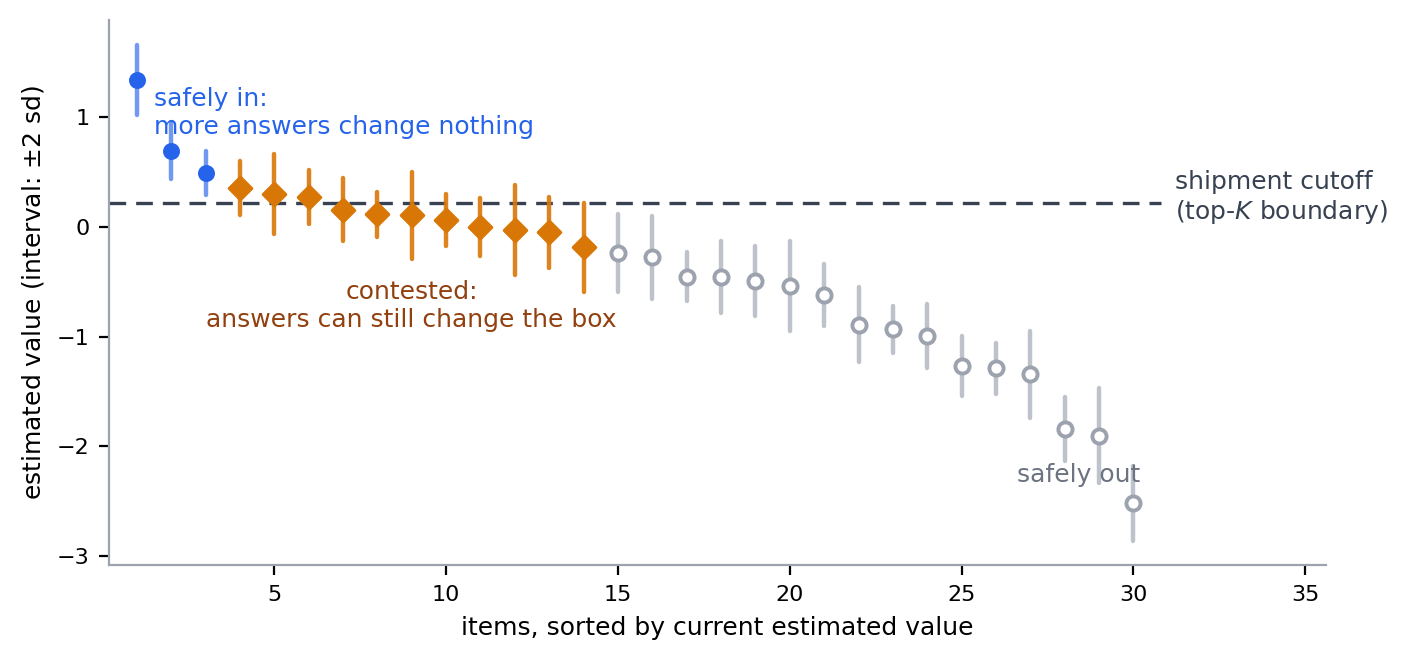
\includegraphics[width=0.92\linewidth]{cutoff_mechanism.png}
\caption{The cutoff mechanism. Items are sorted by current estimated
value, with \(\pm 2\) standard-deviation intervals. Only items whose
intervals straddle the shipment cutoff are contested; answers spent
there can still change the next box, while extra precision on the
safely-in and safely-out groups changes nothing.}
\label{fig:cutoff-mechanism}
\end{figure}

Fix any realization of $(\w,\hat{\w})$. The plug-in rule loses value through the wrong swaps previewed in the
introduction. Products that belong in the oracle box are
left out, and lower-value products are shipped instead. Let $w_{(K)}$
denote the $K$th largest coordinate of $\w$. Every omitted oracle item
has true value at least $w_{(K)}$. Every incorrectly shipped item has
true value at most $w_{(K)}$. Adding and subtracting $w_{(K)}$
re-expresses the loss as
\begin{align}
\sum_{i\in B^*(\w)\setminus \hat B(\hat{\w})} w_i
\;-\;
\sum_{j\in \hat B(\hat{\w})\setminus B^*(\w)} w_j
\;=\;&
\sum_{i\in B^*(\w)\setminus \hat B(\hat{\w})}\big(w_i-w_{(K)}\big)
\notag\\
&\qquad+
\sum_{j\in \hat B(\hat{\w})\setminus B^*(\w)}\big(w_{(K)}-w_j\big).
\label{eq:cutoff-margins}
\end{align}
The next lemma makes the cutoff logic explicit. If estimates are
accurate enough to separate the true cutoff, the platform ships the same
box as the oracle. When a mistake does occur, it must come from a pair of
products whose true values are close enough for estimation error to blur
the cutoff.

\begin{lemma}[Wrong swaps require near-cutoff errors]
\label{lem:wrong-swap-band}
Fix \(\w\) and \(\hat{\w}\), and let
\(\delta=\norm{\w-\hat{\w}}_\infty\). If the true cutoff margin
\(w_{(K)}-w_{(K+1)}\) is larger than \(2\delta\), then the plug-in and
oracle top-\(K\) boxes coincide. More generally, let
\(M=B^*(\w)\setminus \hat B(\hat{\w})\) be the omitted oracle items and
\(I=\hat B(\hat{\w})\setminus B^*(\w)\) the incorrectly included items. If
\(M\) is nonempty, then for any bijection \(\pi:M\to I\),
\[
0\le w_i-w_{\pi(i)}\le 2\delta
\qquad\text{for every }i\in M.
\]
\end{lemma}

Equation~\eqref{eq:cutoff-margins} and
Lemma~\ref{lem:wrong-swap-band} give the section's main lesson. A swap
matters when it replaces an item above the cutoff with one below it. If
beliefs are accurate enough to separate the products around the cutoff,
the wrong swap disappears; when mistakes remain, estimation error has
blurred products on opposite sides of the shipment cutoff. The
managerial implication is direct. Feedback is valuable when it reduces
uncertainty for products that can still enter or leave the box, while
extra precision about clear winners or clear noncontenders rarely
changes the top-\(K\) decision. The next subsection makes this
quantitative.

\subsection[Main characterization of the decision gap]{Main characterization of the decision gap}
\label{subsec:bound-N}

The wrong-swap argument points to the shipment cutoff. The next result
turns that argument into an exact accounting of the proxy gap. It says
which items carry the decision loss, and through which forces. To state it, recall
that \(\kappa_i\) summarizes how much one completed ordinal rating
teaches about item \(i\) (Section~\ref{subsec:estimator}), and that
\(A(\N)\) is the residual proxy covariance after collecting \(\N\)
responses (Section~\ref{subsec:proxy}). When the prior treats product
values as independent, write \(\tau_i\) for the prior precision of item
\(i\), that is, \(\tau_i:=(\bSigma^{-1})_{ii}\). Then
\(a_i(\N):=(\tau_i+\kappa_i N_i)^{-1}\) is the uncertainty that remains about item \(i\) after its \(N_i\) answers.

One more object is needed to say how often an item matters for the decision. For
\(t\in[0,1]\), let \(X_t\sim\mathcal N\big(\bmu,\
\bSigma-(1-t)A(\N)\big)\) denote the proxy vector partway through
learning. At \(t=0\) the platform has only the planned feedback. At
\(t=1\) it has full knowledge.
Under \(X_t\), let \(T_{i,t}\) be the cutoff faced by item \(i\),
namely the \(K\)th largest value among the other items, and let
\(f_{i,t}\) be the density of item \(i\)'s own value.

\begin{proposition}[Decision value of cutoff uncertainty]
\label{prop:gaussian-gap}
The proxy decision gap \(\Delta(\N)\) is nonnegative for every prior
covariance and depends on feedback only through the residual proxy
covariance \(A(\N)\). If the prior is independent, the gap is exactly
\[
\Delta(\N)
\;=\;
\sum_{i=1}^L c_i(\N)\,a_i(\N),
\qquad
c_i(\N)
\;=\;
\frac12\int_0^1 \E\!\big[f_{i,t}(T_{i,t})\big]\,dt
\;\ge\;0.
\]
\end{proposition}

Proposition~\ref{prop:gaussian-gap} is an exact identity, and it gives
the section's main takeaway. Each item contributes the product of
the two forces and nothing else. The factor \(a_i(\N)\) is the
uncertainty the platform has not yet resolved about item \(i\); it
falls as the item receives more informative answers, steeply for the
first answers and more slowly thereafter. The weight \(c_i(\N)\) is the
item's chance of being pivotal. Averaged over the learning path, it is
the probability density with which item \(i\) lands exactly at the
cutoff formed by the other items. For an item whose value distribution
sits far from the cutoff, this density fades at a Gaussian rate. This
is the formal sense in which decision loss concentrates near the
shipment cutoff. An item far from the cutoff can be arbitrarily uncertain and still contribute almost nothing. The same uncertainty attached to a contested item is costly.

The weight \(c_i(\N)\) should not be read as a second uncertainty term.
Feedback can move it, by changing where the cutoff is likely to fall,
but the direct learning effect of assigning more answers to item \(i\)
is carried entirely by \(a_i(\N)\).

With correlated products, the item-by-item formula no longer captures
the whole story, because one response can clarify several related
products near the cutoff. The general statement remains exact. For any
prior covariance, the gap still accumulates nonnegative cutoff terms
along the same learning path (Appendix Proposition~\ref{prop:sep}). The
value of remaining uncertainty then runs through the full residual
covariance \(A(\N)\).
Section~\ref{sec:alloc_opt} uses the local version of the pivot weight,
denoted \(b_i(\N)\), for the marginal value of one additional response
at the current allocation.

The results above are exact for the Gaussian information proxy. The
ordered-probit model enters through the per-answer information
\(\kappa_i(S)\), which calibrates the proxy's observation channel. A
numerical audit compares the proxy posterior mean with the exact
ordered-probit posterior mean. The two agree closely at moderate
response counts, and the audit shows where they diverge at very low ones
(Appendix~\ref{app:surrogate-fidelity}).

Together, these results give an exact account of where feedback is
valuable, but they do not yet specify an allocation policy. The two
design levers turn the account into decisions.
Section~\ref{sec:feedback_design} chooses the format that creates the
information, and Section~\ref{sec:alloc_opt} spends it, one answer at a
time, on the products this section has identified.

\section{Choosing the Feedback Format}
\label{sec:feedback_design}

Before the next box is curated, the platform must commit to one feedback
format. The stakes are documented. Longer or more demanding
questionnaires reduce completion, and major platforms have simplified
rating scales to preserve response rates
\citep{Krosnick1991,Galesic2009,Rolstad2011,FanYan2010,YouTube2009,Netflix2017}.

The results in Section~\ref{sec:gap-analysis} say how to judge the
choice. What matters is the information expected from each exposed
customer, meaning each customer who is shown the questionnaire. Raw
question counts and scale richness are not enough on their own. This
section develops Effective Information Supply (EIS), which measures
exactly that quantity, ahead of the allocation step in
Section~\ref{sec:alloc_opt}.

\subsection{The format decision}
\label{subsec:design-problem}

We study one format shown to customers in a curation segment during a
given box cycle. The platform chooses two features. The first is how many items each customer
rates, denoted by \(Q\). The second is which response scale to use,
denoted by \(S\), the number of ordered response categories.
Together the two features determine how many answers arrive before the
next top-\(K\) decision and how much information each answer carries.

Each feature maps to one observable input. Completion is captured by
\(\alpha(Q,S)\in[0,1]\), the expected fraction of exposed customers who
finish a questionnaire with length \(Q\) and scale \(S\). Completion must be treated as an outcome of the interaction. Feedback is a voluntary customer contribution, and longer
or more demanding instruments reduce participation
\citep{VerhoefReinartzKrafft2010,VanDoornEtAl2010,PansariKumar2017,Krosnick1991,TourangeauConradCouper2013,DillmanSmythChristian2014,Callegaro2015,RevillaSarisKrosnick2014}.
Information per completed answer is captured by \(\kappa_i(S)\) from
Section~\ref{subsec:estimator}. In many menus, completion falls as either feature becomes more
demanding, while richer scales teach more per completed answer. The comparison below does not rely on this pattern.
It needs only the estimated completion and per-answer information of
each candidate format.

With \(T\) exposed customers, a format \((Q,S)\) generates an expected
response budget of
\[
N_{\mathrm{tot}}(Q,S)=T\,Q\,\alpha(Q,S)
\]
recorded answers. The budget is divided across items, with \(N_i\)
answers going to item \(i\). Let \(Q_{\max}\) denote the operational
questionnaire-length limit. For post-consumption ratings of shipped
items one may set \(Q_{\max}=K\). For pre-shipment preference prompts
or hybrid designs, it is the limit imposed by the customer experience.
The question for this section is how to compare
candidate formats on these two inputs before any answers arrive. The
rest of the section puts completion and per-answer information on a
common usable-information scale, so the platform can screen feasible
formats before turning to allocation.

\subsection{Effective Information Supply as a sufficient index}
\label{subsec:eis}

Comparing formats requires a common unit that counts both the number of
answers received and the information in each answer.

For any scale \(S\), let
\[
\bar{\kappa}(S):=\frac{1}{L}\sum_{i=1}^L \kappa_i(S)
\]
be the average per-answer information under that scale. Fix a baseline
scale \(S_0\), such as binary feedback, and define the relative
information multiplier
\begin{equation}\label{def_beta}
\beta(S)\ :=\ \frac{\bar{\kappa}(S)}{\bar{\kappa}(S_0)}.
\end{equation}
Thus \(\beta(S_0)=1\), and \(\beta(S)>1\) means that a completed answer
under scale \(S\) is more informative than a completed answer under the
baseline scale. The EIS comparison uses the multiplier estimated for
each candidate scale; it does not require richer scales to have a larger
multiplier.

\begin{definition}[Effective Information Supply (EIS)]
\label{def:eis}
Let $Q\in\{1,\ldots,Q_{\max}\}$ be the questionnaire length and
$S\in\mathcal S_{\mathrm{cand}}$ a candidate response scale. Let
$\alpha(Q,S)\in[0,1]$ denote the expected completion rate for a
questionnaire with length $Q$ and scale $S$, and let $\beta(S)>0$ be
the relative per-answer information multiplier in \eqref{def_beta}. The
\emph{Effective Information Supply} of format $(Q,S)$ is the expected
number of baseline-answer units generated by one exposed customer,
\[
\mathrm{EIS}(Q,S)\ :=\ \beta(S)\,Q\,\alpha(Q,S).
\]
\end{definition}

For example, a five-question binary format with completion rate \(0.68\)
supplies \(5\times0.68=3.40\) baseline-answer units per exposed customer.
A five-point format with the same length, completion rate \(0.52\), and
information multiplier \(1.35\) supplies
\(1.35\times5\times0.52=3.51\) units. The richer format receives fewer
completed answers but produces slightly more usable information.

When does this product fully determine format choice? The key condition
is that changing the response scale acts like a common information multiplier across products,
\[
\kappa_i(S)=\kappa_i(S_0)\,\beta(S).
\]
Under this factorized information model, a format changes the total
supply of information but not its relative value across products. To
state the result, define the value of a format when its expected response
budget is allocated as well as possible. Using the Gaussian proxy from
Section~\ref{subsec:proxy}, let
\begin{equation}
\label{eq:joint-design-allocation-original}
V^\star(Q,S)
\;:=\;
\max_{\N\ge0}\;
\E\!\big[V_K(\tilde{\w}(\N))\big]
\quad\text{subject to}\quad
\sum_{i=1}^L N_i\le T\,Q\,\alpha(Q,S),
\end{equation}
where per-answer information is \(\kappa_i(S)\). This is the best
expected next-box value the platform can reach with format \((Q,S)\).

\begin{proposition}[Feedback-design decomposition under factorized information]
\label{prop:eis-equivalence}
Under the factorized information model
$\kappa_i(S)=\kappa_i(S_0)\,\beta(S)$ with \(\beta(S_0)=1\), fix $T$ and
a feasible menu of candidate formats, and let $V^\star(Q,S)$ be the
format-optimized value in \eqref{eq:joint-design-allocation-original}. Then there exists a
format-invariant, nondecreasing scalar value function \(\Psi\) such that,
for every candidate format,
\[
V^\star(Q,S)=\Psi\!\big(T\cdot \mathrm{EIS}(Q,S)\big).
\]
\end{proposition}

Proposition~\ref{prop:eis-equivalence} is the reason for using EIS.
Under factorized information, two formats that generate the same EIS
give the platform the same total information budget, measured in
baseline-answer units. After this rescaling, the allocation problem is
the same regardless of which format produced the budget. The best
achievable next-box value therefore depends on \((Q,S)\) only through
\(T\cdot\mathrm{EIS}(Q,S)\).

Within this model, EIS is an exact index for format choice. Any format
that maximizes EIS also maximizes the expected value of the optimized
next-box decision. The model is the deterministic expected-budget,
continuous-allocation relaxation. Completion counts are binomial and
answers are integers, and with many exposed customers the relaxation is
the standard fluid approximation. The platform can therefore rank formats before solving the
product-level allocation problem. When scale changes affect products by
different proportions, EIS no longer guarantees an exact ranking. It
then serves as a first screen, with close formats reserved for a larger
pilot or the full allocation problem. The next subsection explains how
to estimate the inputs and assess these departures.

\subsection{Calibrating and using EIS}
\label{subsec:eis-practical}

The metric becomes operational once the platform estimates two inputs
for each candidate format. The first is completion,
\(\alpha(Q,S)\), the share of exposed customers who submit the requested
answers. If partial responses are usable, the platform can instead use
the expected number of submitted ratings. The second is \(\beta(S)\),
the information in one completed answer relative to a baseline scale. A
clean pilot estimates both quantities on the same exposed population,
using randomized formats and common calibration items when feasible.

Both inputs are observable in standard pilot data. Completion comes from
exposure and submission logs. The platform can estimate relative
information by fitting the same ordinal-response model under each scale
and comparing how much one answer reduces posterior uncertainty. Pilot
resampling can then provide uncertainty bands for EIS, which matter when
two formats are close.

\paragraph{Illustration with public inputs.}
Table~\ref{tab:eis-calibrated} illustrates the calculation with public
inputs. The information multiplier is fitted from
MovieLens ratings \citep{HarperKonstan2016}. We fit ordered-probit
cutpoints to the pooled rating distribution, recover item values for
the 200-item catalog of Section~\ref{subsec:numerics_movielens}, and
average the resulting per-answer information. This gives \(\hat\beta(5)=1.49\), close to the \(1.35\) used above.

Completion is pinned to the response-rate benchmarks cited in the introduction
\citep{Malnik2025}. The lightest format completes at \(0.29\) and the
heaviest at \(0.13\), with a log-linear decline in questionnaire burden
between the two anchors. The log-linear shape has experimental support.
In the randomized length experiment of \citet{Galesic2009}, completion
fell from \(68\) to \(57\) to \(47\) percent as announced length rose
from ten to twenty to thirty minutes, an almost constant log decline
per added minute. Large observational evidence points the same way. Across more than \(25{,}000\) real web surveys, completion falls only
from \(89\) to \(79\) percent between ten and forty questions
\citep{LiuWronski2018,SurveyMonkeyCompletion2020}. Within a three-to-seven prompt menu, the
question-count effect is therefore mild.

Scale burden is a separate force, and the evidence on it spans a wide
range. In survey settings, the burden of a richer scale is modest. In Netflix's in-product test, by contrast, thumbs collected about three
times as many ratings as five-star prompts \citep{Netflix2017}.
Table~\ref{tab:eis-calibrated} therefore reports two completion
scenarios with the same fitted multiplier. Under survey-like burden,
the five-point \(Q{=}5\) format leads, because the richer answers
outweigh the completion loss. Under in-product burden, with the Netflix ratio
applied to the five-point formats, the ranking flips and the binary
\(Q{=}5\) format leads. The flip is the point. Both scenarios are
documented, and which one a platform faces is an empirical question
about its own prompts and audience. EIS turns that empirical trade-off
into a format comparison. Within the survey scenario, the cited
benchmarks do not identify the additional burden of a richer scale.
Varying that burden over a wide range moves the leading EIS values by
several percent but does not lift a binary format to the top of that
scenario.

\begin{table}[H]
\centering
\scriptsize
\setlength{\tabcolsep}{5pt}
\begin{tabular}{lccccc}
\toprule
 & & \multicolumn{2}{c}{Survey burden} & \multicolumn{2}{c}{In-product burden} \\
\cmidrule(lr){3-4}\cmidrule(lr){5-6}
Format & Fitted \(\hat\beta(S)\) & \(\alpha\) & EIS & \(\alpha\) & EIS \\
\midrule
Binary, $Q=3$  & $1.00$ & $0.290$ & $0.87$ & $0.290$ & $0.87$ \\
Binary, $Q=5$  & $1.00$ & $0.219$ & $1.10$ & $0.219$ & $\mathbf{1.10}$ \\
5-point, $Q=3$ & $1.49$ & $0.261$ & $1.17$ & $0.097$ & $0.43$ \\
5-point, $Q=5$ & $1.49$ & $0.184$ & $\mathbf{1.38}$ & $0.073$ & $0.55$ \\
5-point, $Q=7$ & $1.49$ & $0.130$ & $1.36$ & $0.055$ & $0.58$ \\
\bottomrule
\end{tabular}
\caption{Calibrated EIS profiles under the two completion scenarios described in the text. The information multiplier is fitted from MovieLens 100K. Bold marks the leader in each scenario; EIS values are computed from unrounded inputs.}
\label{tab:eis-calibrated}
\end{table}

Table~\ref{tab:eis-calibrated} illustrates why neither format length nor
scale richness is enough on its own. Richer formats lead when their
information advantage outweighs the completion loss; leaner formats lead
when completion is more sensitive to burden. The comparison that matters
is the expected baseline-equivalent information per exposed customer.

The factorization condition also explains when the catalog average in
\eqref{def_beta} is sufficient. If a scale change multiplies every
item's information by the same factor, uniform and cutoff-weighted
averages produce the same \(\beta(S)\) and the same format ranking. When
the ratios vary across items, the products near the cutoff deserve more
weight. In the MovieLens calibration, the item-level ratios deviate from exact
factorization by about ten percent. Section~\ref{subsec:eis-screening}
measures the resulting ranking error directly. A platform can run the
same item-level diagnostic in a pilot and send close format comparisons
to the full allocation model.

\paragraph{Choosing a format.} For each candidate \((Q,S)\), compute
\[
\widehat{\mathrm{EIS}}(Q,S)=\hat\beta(S)Q\hat\alpha(Q,S),
\]
or use the expected number of submitted ratings when partial completions
are counted. If one format is clearly separated and satisfies operational
guardrails such as maximum length, minimum completion, and implementation
cost, it is the natural candidate to deploy. If the leading formats are statistically close, EIS shortlists a few
candidates for a larger pilot.

The same procedure can be adapted to less controlled data. Randomized
pilots give the cleanest ranking for the tested menu. With observational
logs, the completion and information estimates should be treated as
forecasts and checked on holdout data. When one common format must
serve several known segments, the platform can estimate completion and
per-answer information separately for each segment. A candidate format is then screened by the traffic-weighted average of
its segment scores. The average is a screen. When segments respond very
differently, close calls need the segment-level comparison.

Whatever format wins, it hands the allocation step two objects, an expected response budget \(N_{\mathrm{tot}}=T\,Q\,\alpha(Q,S)\) and a
per-answer information level \(\kappa_i(S)\).
Section~\ref{sec:alloc_opt} decides where that budget goes.

\section{Allocating Answers After the Format Is Chosen}
\label{sec:alloc_opt}
Section~\ref{sec:feedback_design} chooses the feedback format. Once that
choice is fixed, the platform has a limited supply of answers to spend
before the next box is curated. The question is where the next answer is
most likely to improve the shipment decision.

The answer follows the cutoff logic from
Section~\ref{sec:gap-analysis}. The same two forces reappear. A product is a valuable feedback target when its box membership is still
contested and when another answer can still teach the platform
something. This section turns these forces into a fixed-format
allocation rule. The section states the fixed-format benchmark, derives the value of one more answer, and turns it into the operating scores used in Section~\ref{sec:numerics}.

\subsection{Fixed-format allocation problem}
\label{subsec:alloc-preamble}
\label{subsec:alloc-objective}

The format step fixes an expected budget of \(N_{\mathrm{tot}}\)
recorded answers and a per-answer information level \(\kappa_i\) for
each product under the chosen scale (Section~\ref{subsec:design-problem}). When partially completed questionnaires are usable,
\(N_{\mathrm{tot}}\) is the expected number of submitted ratings. The allocation decision is
how to distribute this budget across products. This keeps the two
managerial levers distinct. Section~\ref{sec:feedback_design} chooses a
format that customers will complete. The present section decides where
the resulting answers have the largest decision value.

Two common baselines show what a rule misses when it considers only one
part of the decision. Uniform
allocation treats all products as equally useful learning targets, even
though many products cannot plausibly cross the shipment cutoff.
Uncertainty-only allocation asks about the products with the widest
remaining beliefs, even when those products are far from the cutoff. An
effective rule must combine the two ideas, giving priority to items whose
uncertainty could change the next box.

The fixed-format benchmark needs no new program. It is the allocation
problem inside \eqref{eq:joint-design-allocation-original}, with the
format now fixed. The platform spends at most \(N_{\mathrm{tot}}\)
answers to maximize the expected value of the shipped box. The objective keeps the managerial target visible. The platform
maximizes the expected value of the selected top-\(K\) set. Prediction
accuracy on products that never approach the cutoff earns no credit.
Maximizing this objective is the same as minimizing the decision gap \(\Delta(\N)\)
from Section~\ref{sec:gap-analysis}. Allocation spends the budget where
it removes the most decision loss.

Solving this full problem after every response would be impractical. It
nevertheless identifies the question a usable rule should answer. Given
the current allocation, where would one more answer improve the next-box
decision most?

\subsection{The marginal value of responses}
\label{subsec:alloc-local-value}
\label{subsec:alloc-diagonal-rule}

The fixed-budget benchmark asks for a full allocation. A sequential rule
instead asks where the next response helps most. The next result is the
derivative of the gap in Proposition~\ref{prop:gaussian-gap} with
respect to the allocation, item by item. It is a marginal value in the
continuous allocation relaxation. The value of one full answer is this
derivative integrated over a unit increase in \(N_j\).

\begin{proposition}[Marginal value of responses after format choice]
\label{prop:local-marginal}
Fix a chosen format and a current allocation \(\N\). For any item \(j\),
the marginal value of responses to item \(j\) is
\[
\mathrm{MV}_j(\N)
\;:=\;
\lim_{h\downarrow0}
\frac{\E[V_K(\tilde{\w}(\N+h e_j))]
-\E[V_K(\tilde{\w}(\N))]}{h},
\]
which is nonnegative. If the prior is independent, the marginal value
is exactly
\begin{equation}
\mathrm{MV}_j(\N)
\;=\;
\underbrace{b_j(\N)}_{\text{cutoff relevance}}
\times
\underbrace{\frac{\kappa_j}{(\tau_j+\kappa_jN_j)^2}}_{\text{remaining learnability}},
\label{eq:priority-decomposition}
\end{equation}
where \(b_j(\N)\ge0\) is the local pivot density of item \(j\) at the
shipment cutoff; its formal definition, the closed form for correlated
priors, and the regularization at covariance-boundary points accompany
the proof in the appendix.
\end{proposition}

The weight \(b_j(\N)\) is the local counterpart of the pivot weight
\(c_j(\N)\) in Proposition~\ref{prop:gaussian-gap}. Both measure the
chance that item \(j\) lands at the shipment cutoff. The pivot weight
averages that chance over the learning path. The local weight evaluates
it at the current allocation. The two terms in
\eqref{eq:priority-decomposition} read directly. Cutoff relevance is
large when item \(j\) often lies near the margin between being included
and excluded. The second term is large when the chosen format is
informative and item \(j\) has not already received many
answers. With correlated products, the same derivative also credits a
response about item \(j\) for the related uncertainties it reduces. The vector \(A(\N)e_j\)
records which other products an answer about \(j\)
clarifies, and the response is valuable when those products are
themselves near the shipment cutoff.

The product form also makes precise why uncertainty-only allocation
can mislead. It ranks items by the second term alone, and that
ranking matches the marginal value only when the compared items
are equally close to the shipment cutoff.

\subsection{Operating scores and segment allocation}
\label{subsec:global-solver}

The exact cutoff-density term \(b_i(\N)\) comes from the theory. In an
operating policy, the platform can replace it with a cutoff-proximity
score \(\widehat b_i(\N)\), computed from current product estimates. The
score is high for products close to the current cutoff and low for
products that are clearly in or clearly out. The resulting rule assigns
the next answer to
\[
j\in\arg\max_{i=1,\ldots,L}\;
\widehat b_i(\N)\,
\frac{\kappa_i}{(\tau_i+\kappa_iN_i)^2}.
\]
The first factor asks whether product \(i\)'s box membership is still
contested. The second asks how much one more answer can still teach under
the chosen format. In the numerical policies, we estimate the current cutoff \(\hat
w_{(K)}\) and give each product a proximity score that is highest at the
cutoff and fades with distance. An item's score also fades as it accumulates answers,
because each additional answer about the same item teaches less than the
one before. We call the result the guarded cutoff rule. It is the operating policy the rest of the paper
recommends and tests, and it needs no separate calibration of the
theoretical density \(b_i(\N)\).

The rule is greedy. It spends each next answer where the current
marginal value is highest. A small-scale numerical check measures how
this sequential choice compares with a fixed allocation of the full
budget. With twelve items and direct optimization
over fixed allocations, the exact myopic one-answer policy captures
\(90\) to \(99\) percent of the achievable improvement over even
allocation,
across independent and correlated priors and across tight and generous
budgets (Appendix~\ref{app:greedy-optimal}). The operating score gives up
more, mainly at generous budgets, where allocation matters least. When
the pivot weights are held fixed, the benchmark spreads
answers across the contested items, keeping none of them much more
uncertain than the rest and tilting toward those most likely to be
pivotal. The greedy rule builds that pattern one answer at a time. The
experiments in Section~\ref{sec:numerics} show when this rule is
adequate and when its refinements matter.

This score organizes the policies compared in
Section~\ref{sec:numerics}. Uniform spreads answers evenly across the
catalog. Uncertainty-only keeps the second term and drops cutoff proximity. The
guarded cutoff rule keeps the proximity score and replaces the
learnability term with count damping. The combined rule multiplies
cutoff proximity by remaining posterior uncertainty. An estimated
marginal-value rule computes the marginal value in
Proposition~\ref{prop:local-marginal} from the current posterior. A correlation-aware
variant gives credit to answers that also clarify related products
near the cutoff.

If the platform allocates feedback across several known curation
segments, the unit of allocation becomes a segment-item pair. Segment \(h\) enters with weight \(\pi_h\). The deciding question is
still whether another response can change that segment's next-box
decision. The segment priority is
\[
(\hat h,\hat j)\in\arg\max_{h,j}\;
\underbrace{\pi_h}_{\text{segment weight}}
\times
\underbrace{\widehat b_{hj}(\N)}_{\substack{\text{close to}\\
\text{segment cutoff}}}
\times
\underbrace{\frac{\kappa_{hj}}{(\tau_{hj}+\kappa_{hj}N_{hj})^2}}_{\substack{\text{what one more}\\
\text{answer can teach}}}.
\]
The segment weight scales the value of resolving a segment's decision,
but it does not by itself determine where the next question should go. A
large segment need not receive the next question if its top-\(K\) set is
already clear; a smaller segment can be worth querying when its cutoff
is crowded. With an independent prior, the exact segment formula replaces
\(\widehat b_{hj}\) with the local cutoff-density term \(b_{hj}\). With
correlated products or shared factors, the rule also credits a response
for clarifying related borderline segment-item pairs. Appendix
Proposition~\ref{prop:finite-segments} gives the formal segment version.

After the format is fixed, the next answer should go where it can
still change the box. Section~\ref{sec:numerics} compares the policies
above and shows when uncertainty and correlation refine the primary
cutoff-targeting logic.

\section{Numerical Experiments}\label{sec:numerics}
\subsection{Experimental roadmap and setup}\label{subsec:setup}

The experiments take up four questions in turn. Section~\ref{subsec:design-allocation} measures whether targeting products near the cutoff improves the next box relative to uniform or uncertainty-only allocation. Section~\ref{subsec:sensitivity-scaling} maps when posterior uncertainty, related-product learning, and segment weights improve that simple rule. Section~\ref{subsec:eis-screening} tests whether EIS identifies good feedback formats before any answers arrive. Section~\ref{subsec:numerics_movielens} checks whether the allocation pattern also appears in chronological MovieLens ratings.

We use synthetic experiments when exact evaluation requires known true
product values. Table~\ref{tab:calibration-sources} lists the public or
observational sources used to calibrate the main inputs.

\begin{table}[h!]
\centering
\scriptsize
\setlength{\tabcolsep}{5pt}
\begin{tabular}{lll}
\toprule
Model input & Data source & Enters in \\
\midrule
Information multiplier \(\hat\beta(5)=1.49\) & Fitted to MovieLens 100K ratings & Section~\ref{subsec:eis} \\
Factorization deviation (\(\pm 10\%\)) & Same MovieLens fit, item level & Section~\ref{subsec:eis} \\
Completion levels (\(0.29\), \(0.13\)) & Published response-rate benchmarks & Section~\ref{subsec:eis} \\
Completion shape (log-linear) & Randomized length experiment & Section~\ref{subsec:eis} \\
Question-count slope (mild) & \(25{,}000\) real web surveys & Section~\ref{subsec:eis} \\
Scale-burden ratio (\(\times 3\)) & Netflix in-product test & Section~\ref{subsec:eis} \\
Per-answer information \(\kappa_i(S)\) & Ordered-probit information at fitted cutpoints & Sections~\ref{subsec:design-allocation}--\ref{subsec:eis-screening} \\
Catalog, ratings, decision target & MovieLens 100K, chronological splits & Section~\ref{subsec:numerics_movielens} \\
Box-composition associations with retention & Industrial curation log, author's analysis & Section~\ref{subsec:retention} \\
\bottomrule
\end{tabular}
\caption{Calibrated inputs behind the experiments and their data sources.}
\label{tab:calibration-sources}
\end{table}

We consider a catalog of $L$ items with a Gaussian prior
\[
\w \sim \mathcal{N}(\boldsymbol{\mu},\,\boldsymbol{\Sigma}),\qquad
\boldsymbol{\mu}\in\mathbb{R}^L,\ \boldsymbol{\Sigma}\in\mathbb{S}_{++}^L.
\]
Unless stated otherwise, the prior mean is generated as $\mu_i\stackrel{\text{i.i.d.}}{\sim}\mathcal{N}(0,1)$. The default prior covariance is a correlated AR(1),
\[
(\boldsymbol{\Sigma}_{\text{AR(1)}})_{ij}=\rho^{\,|i-j|}\quad\text{with}\ \rho=0.6,
\]
which lets one response teach the platform about related products. The independent prior $\boldsymbol{\Sigma}=I$ appears where the theory's
closed forms require it and as a reference in the allocation tables. Customer feedback follows the ordered-probit model from Section~\ref{sec:problem-setting}
\[
u_{it}\mid w_i\sim\mathcal N(w_i,1),\qquad
R_{it}=k\ \Longleftrightarrow\ \theta_{k-1}<u_{it}\le \theta_k,\quad
k\in\cR_S.
\]
We study binary and five-category scales, \(S\in\{2,5\}\), with
centered thresholds.

We use the ordinal channel in two ways. The EIS exercise computes
ordered-probit information directly. The allocation experiments use the
Gaussian information-equivalent channel from Section~\ref{subsec:proxy}. An
additional response on item \(i\) is represented by a normal signal with
variance \(1/\kappa_i(S)\), where \(\kappa_i(S)\) is the ordered-probit
Fisher information for the chosen scale. This keeps the allocation
experiments aligned with the exact Gaussian-proxy theory while leaving
the ordered-feedback bridge visible.

The surrogate $\tilde{\w}$ gives a fast deterministic approximation to
the full ordinal-probit posterior mean and avoids posterior sampling in
the large allocation experiments. Appendix~\ref{app:surrogate-fidelity}
reports the audit behind this choice. Against a data-augmentation
posterior mean, the top-\(K\) sets induced by the surrogate overlap by
\(95\%\) to \(100\%\) at ten or more responses per item; a low-count extension in the same appendix shows where the approximation
frays. All allocation policies use the same surrogate from the same five-
response warm start. The common surrogate keeps the comparison
controlled within the proxy model; it does not by itself establish that
the policy ranking is invariant to exact ordinal updating at very low
counts. The remaining subsections turn to the design questions.

\subsection[Where to spend scarce answers]{Where to spend scarce answers near the cutoff}\label{subsec:design-allocation}

This is the main allocation experiment. After the platform has a small
amount of baseline feedback, is it better to spend new responses near
the shipment cutoff than to spread them evenly or chase uncertainty
alone? The centerpiece is the guarded cutoff rule of
Section~\ref{subsec:global-solver}, the operating policy this paper
recommends. We fix $(L,K)=(60,6)$, so each world curates a box of six
items from a sixty-item catalog. Each recorded answer carries the
information of a five-category rating, through the Gaussian channel
described above. Five policies compete at the same three budgets,
\(N_{\mathrm{tot}}\in\{10L,30L,100L\}\), that is, an average of ten to
one hundred answers per catalog item.

The five policies differ only in how they pick the next item to ask
about. Our method is the guarded cutoff rule. It asks about items near
the current shipment cutoff and gradually loses interest in items it
has already queried many times. Two simpler baselines ignore part of
the decision. Even allocation spreads answers uniformly across the
catalog, and uncertainty-only targeting asks about the item whose
answer would reduce total posterior variance most, wherever that item
sits. Two richer alternatives estimate what our rule approximates. The
combined cutoff \(\times\) uncertainty rule keeps the cutoff focus but
measures remaining learnability from the posterior instead of from
response counts, and the estimated marginal-value rule implements the
priority formula of Proposition~\ref{prop:local-marginal} directly.

\paragraph{Implementation.}
The functional forms are deliberately generic and the constants are
round defaults. Let \(\hat c=\hat w_{(K)}\) be the current estimated cutoff and let the proximity score of item \(i\) be
\[
k_i \;=\; 0.10+0.90\exp\!\big(-\big((\hat w_i-\hat c)/h\big)^2\big),
\qquad
h=\max\{\mathrm{med}(g_K),\,0.10\,\mathrm{sd}(\hat{\w}),\,0.08\},
\]
where \(g_K\) holds the two order-statistic gaps adjacent to the cutoff, \(\hat w_{(K-1)}-\hat w_{(K)}\) and \(\hat w_{(K)}-\hat w_{(K+1)}\), and \(\mathrm{sd}(\hat{\w})\) is the cross-sectional standard deviation of the current means. The guarded cutoff rule queries \(\arg\max_i k_i/(1+0.10\,N_i)\), where \(N_i\) is the number of answers item \(i\) has received; we call the division the count damping. It keeps the rule from spending the whole budget on the same few borderline items, since each answer an item receives shrinks its score, halving it after ten. In the language of Proposition~\ref{prop:local-marginal}, which prices an answer as cutoff relevance times what is left to learn, the count damping is a shortcut for the second factor; the combined and marginal-value rules estimate that factor from the posterior instead, and their exact scores are in Appendix~\ref{app:refinement-tables}. All constants were chosen once during development and held fixed across every experiment, both priors, and all budgets.

The experiment uses a common warm start of five responses per item and
\(100\) shared synthetic worlds, each a fresh draw of true item values
and response noise. Table~\ref{tab:alloc-efficacy} reports mean
next-box value gaps with standard errors, and
Figure~\ref{fig:policy-gaps} plots them. The replication package
reports the world-level raw outcomes, win rates, and paired
improvements behind both.

\begin{table}[h!]
\centering
\scriptsize
\setlength{\tabcolsep}{4pt}
\begin{tabular}{lcccccc}
\toprule
Prior & $N_{\mathrm{tot}}$ & \shortstack{Guarded\\cutoff} & Even & Uncertainty-only & \shortstack{Combined cutoff\\$\times$ uncertainty} & \shortstack{Estimated\\marginal value} \\
\midrule
AR(1) $\rho=0.6$            & $10L$   & $\mathbf{0.078}\,(0.013)$ & $0.297\,(0.033)$ & $0.251\,(0.033)$ & $0.111\,(0.016)$ & $0.083\,(0.015)$ \\
AR(1) $\rho=0.6$            & $30L$   & $\mathbf{0.022}\,(0.006)$ & $0.138\,(0.017)$ & $0.127\,(0.019)$ & $0.062\,(0.011)$ & $0.061\,(0.012)$ \\
AR(1) $\rho=0.6$            & $100L$  & $\mathbf{0.008}\,(0.002)$ & $0.045\,(0.007)$ & $0.048\,(0.008)$ & $0.017\,(0.004)$ & $0.042\,(0.010)$ \\
\midrule
Independent ($\bSigma{=}I$) & $10L$   & $\mathbf{0.107}\,(0.017)$ & $0.400\,(0.037)$ & $0.363\,(0.037)$ & $0.119\,(0.017)$ & $0.113\,(0.018)$ \\
Independent ($\bSigma{=}I$) & $30L$   & $\mathbf{0.035}\,(0.009)$ & $0.209\,(0.025)$ & $0.151\,(0.018)$ & $0.050\,(0.009)$ & $0.080\,(0.015)$ \\
Independent ($\bSigma{=}I$) & $100L$  & $\mathbf{0.004}\,(0.001)$ & $0.050\,(0.010)$ & $0.055\,(0.010)$ & $0.022\,(0.005)$ & $0.061\,(0.014)$ \\
\bottomrule
\end{tabular}
\caption{Mean next-box value gaps under alternative ways to spend the same response budget over \(100\) shared synthetic worlds. Lower values are better; bold marks the best policy in each row.}
\label{tab:alloc-efficacy}
\end{table}

\begin{figure}[t]
\centering
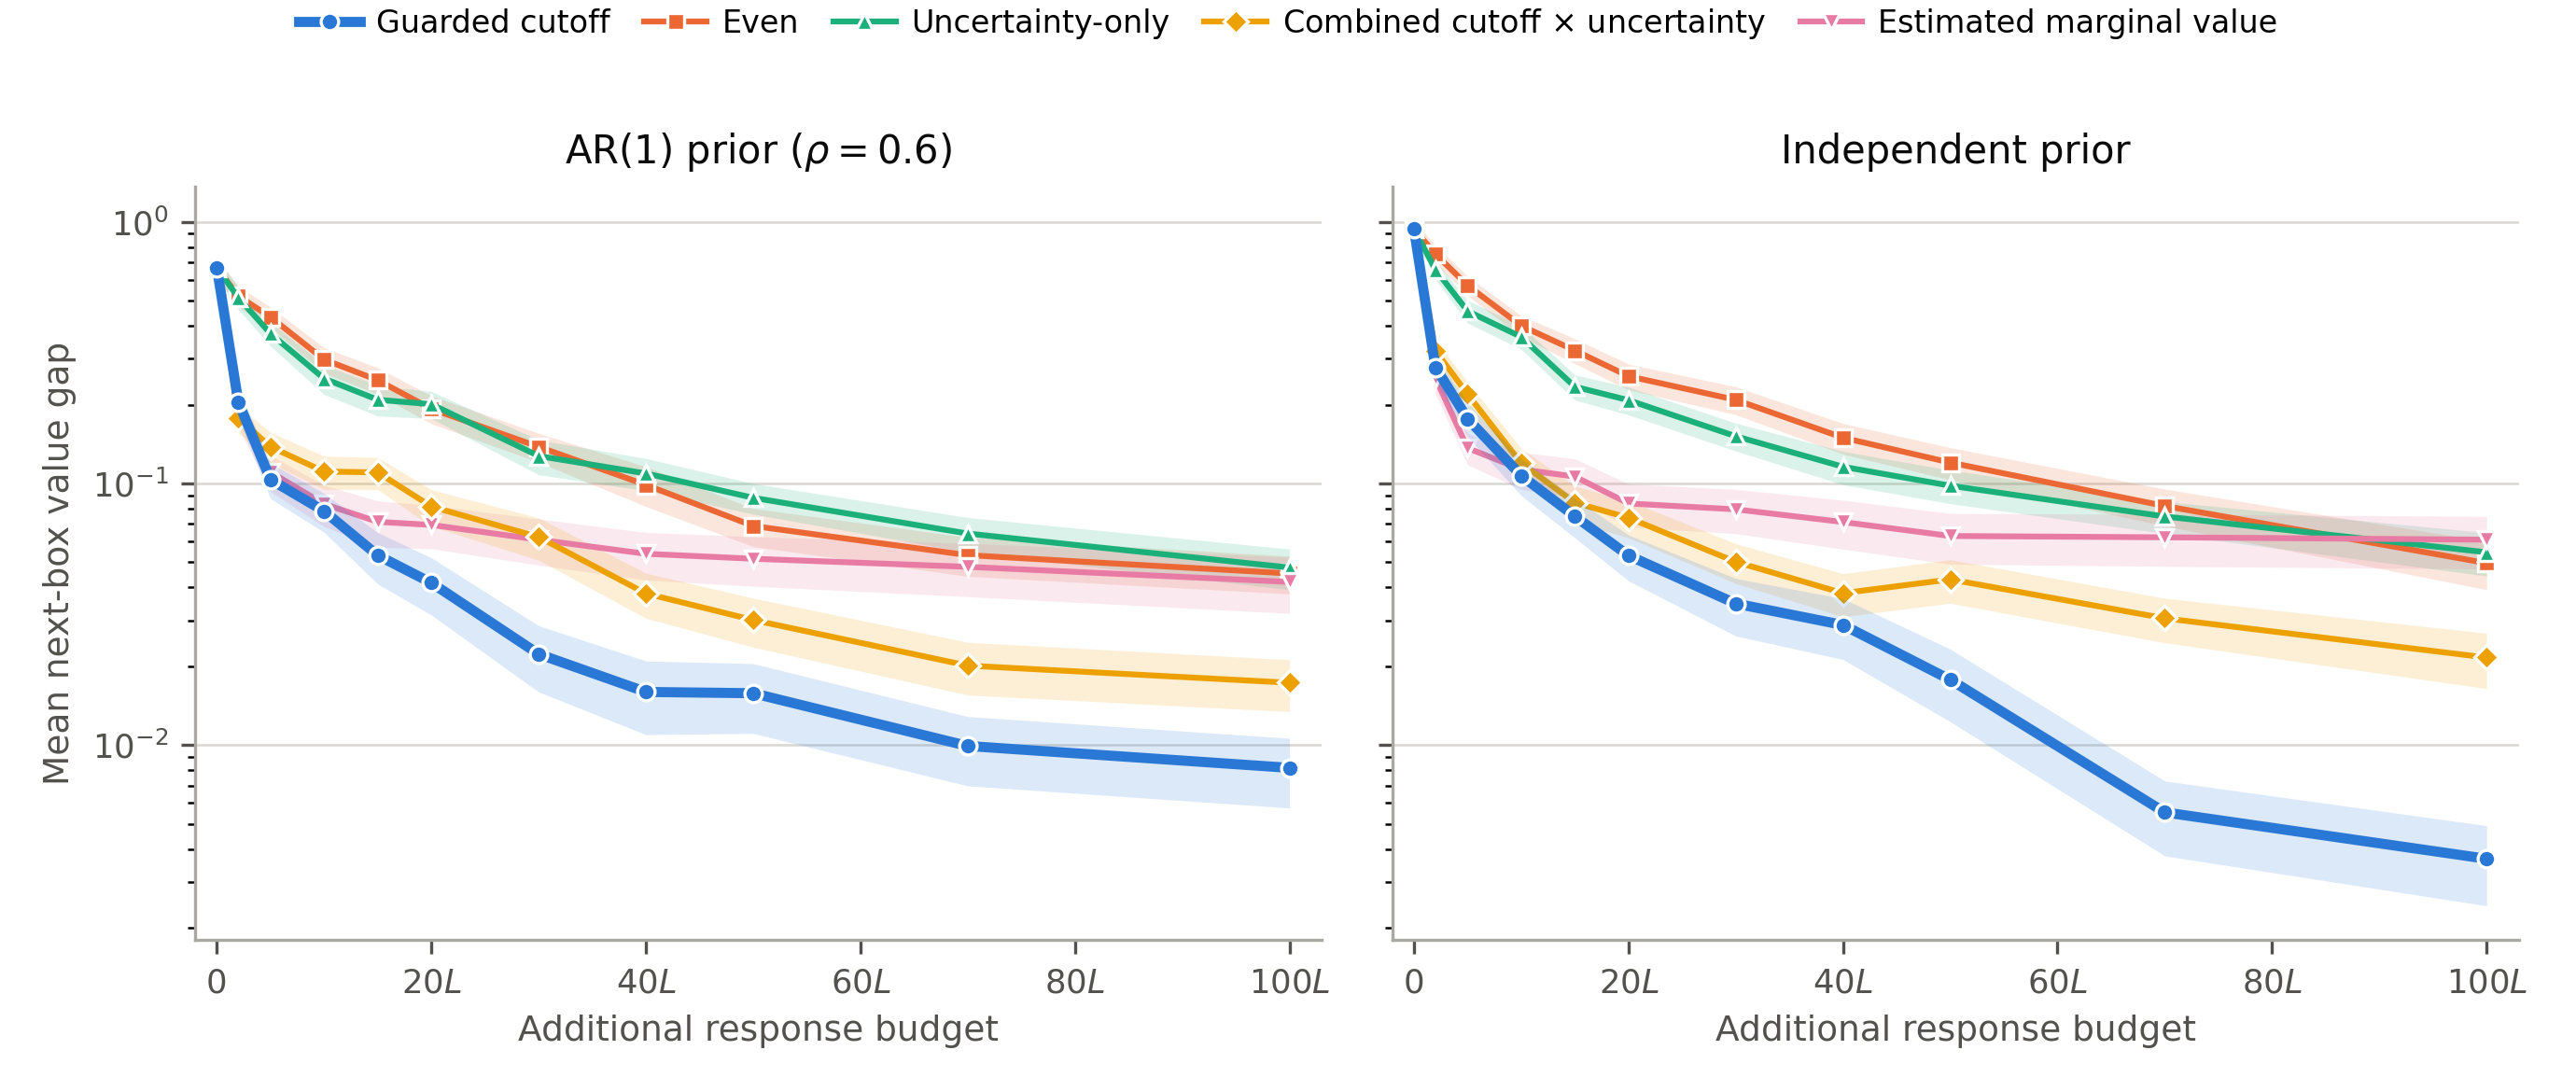
\includegraphics[width=\textwidth]{policy_gap_comparison.png}
\caption{Mean next-box value gaps by policy and response budget (log
vertical scale; lower is better). Budget \(0\) is the shared
five-response warm start, and shaded bands are one standard error over
the \(100\) worlds. The guarded cutoff rule attains the lowest gap at
every budget under both priors.}
\label{fig:policy-gaps}
\end{figure}

The guarded cutoff rule has the lowest mean gap in all six
prior-budget settings and the smallest gap in \(65\) to \(90\) percent
of individual worlds (Appendix Table~\ref{tab:alloc-win-rates}).
Cutoff relevance carries most of the allocation value. Uncertainty-only targeting is weak in both prior structures because it
keeps uncertainty while ignoring whether that uncertainty can change the
next box. The margin also holds against the closest off-the-shelf
method. A sequential OCBA-m rule from ranking and selection
\citep{ChenHeFuLee2008} loses to the guarded rule at every budget under
both priors (Appendix Table~\ref{tab:ocba}).

Removing the count damping shows why it is there. Without it the rule
keeps querying the same near-cutoff items, and its gap stays flat at
\(0.30\) to \(0.43\) as the budget grows tenfold, while the guarded
rule falls to \(0.008\) (replication package). The guarded cutoff rule
is thus itself a two-factor rule in the sense of
Proposition~\ref{prop:local-marginal}, cutoff relevance times a robust
form of diminishing returns, and the columns of
Table~\ref{tab:alloc-efficacy} compare implementations of the second
factor. Counts prove sturdier than posterior estimates at large
budgets.

A sharper test runs the myopic ideal exactly. Under the independent
prior, the expected gain from one full answer has a closed form, so the
rule that always takes the highest one-answer gain needs no proximity
score and no estimation. It stalls. Its gap sits at \(0.097\) at every
budget while the guarded rule falls from \(0.073\) to \(0.006\) on the
same worlds (Appendix~\ref{app:greedy-optimal}). The reason is
short-sightedness. An item whose mean is confidently wrong offers a
negligible one-answer gain, so it is never queried and the mistake
becomes permanent. Exploration, here the score floor and the count
damping, is what a practical rule must add. On the same benchmark, the
guarded rule also achieves a lower mean gap than the best static
allocation found by direct optimization at every budget.

The estimated marginal-value rule shows the practical role of
Proposition~\ref{prop:local-marginal}. It is competitive at the tight
\(10L\) budget and falls behind as the budget grows, at \(100L\) even
behind even allocation. Cutoff relevance sets the priority; the
posterior refinements matter only when near-cutoff items differ in what
is left to learn.

\subsection[When to refine cutoff targeting]{When to refine cutoff targeting}\label{subsec:sensitivity-scaling}

The main allocation result says that cutoff relevance should receive
the most weight. This subsection summarizes when the simple rule should be refined.
Figure~\ref{fig:refinement-map} maps the central boundary, and
Appendix~\ref{app:refinement-tables} reports the full tables.

\begin{figure}[t]
\centering
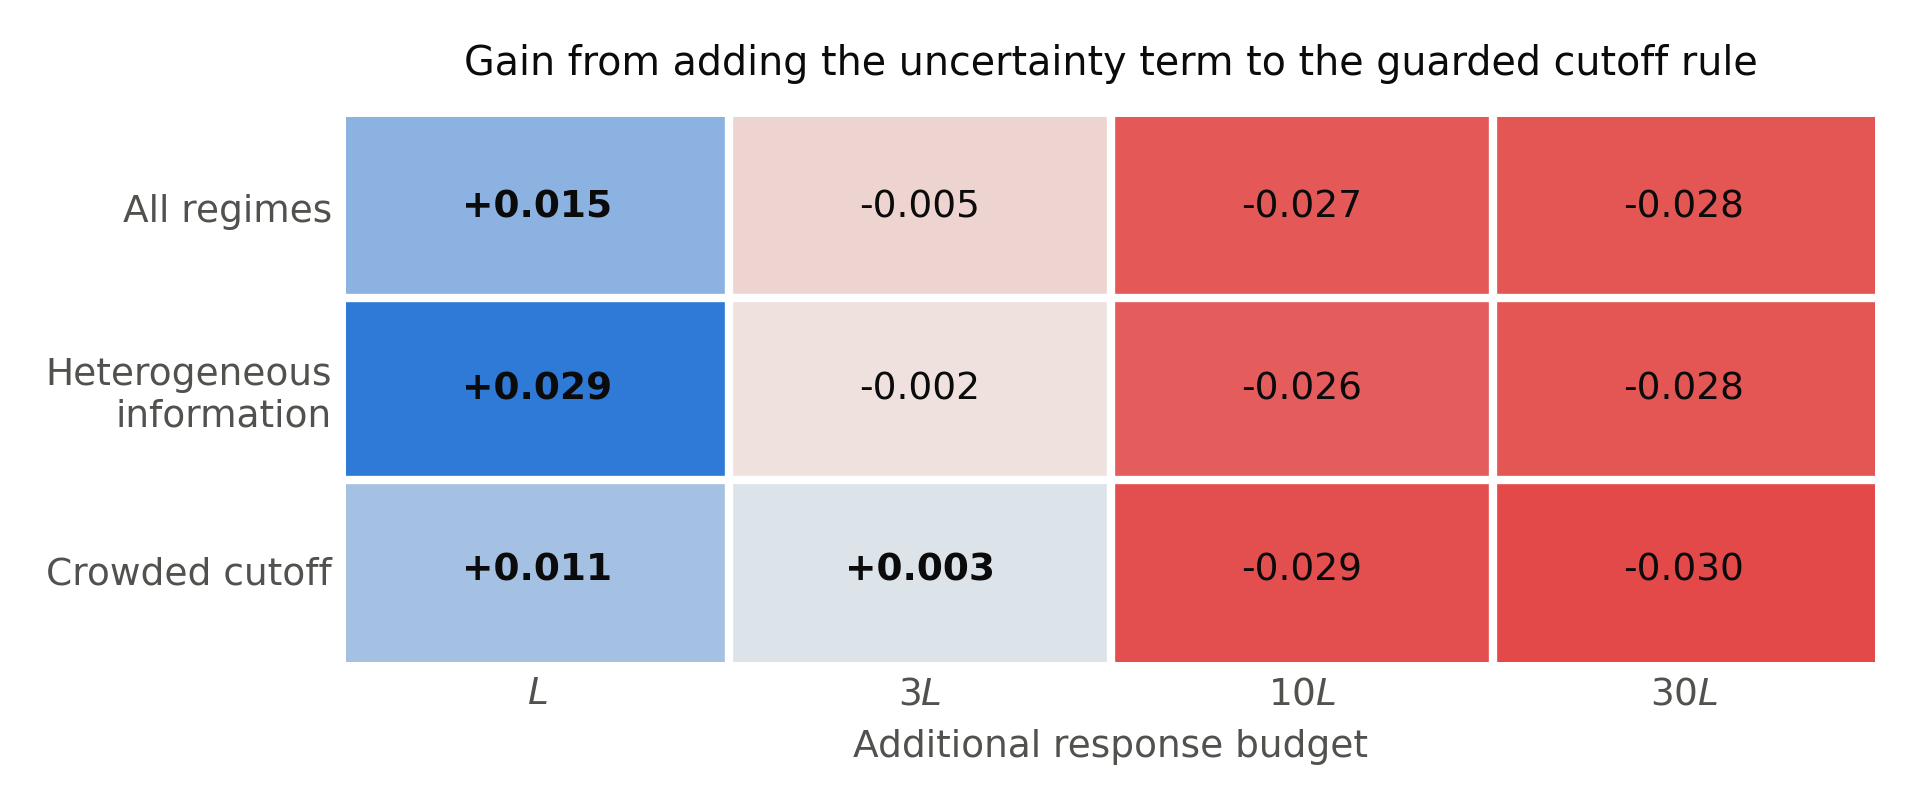
\includegraphics[width=0.82\textwidth]{refinement_boundary_map.png}
\caption{The refinement boundary. Each cell is the mean improvement of
the combined cutoff \(\times\) uncertainty rule over the guarded
cutoff rule, by response budget and scenario group, aggregated over the
regime map of Appendix~\ref{app:refinement-tables}. Blue cells mean
the uncertainty term helps; red cells mean the guarded rule alone is
better.}
\label{fig:refinement-map}
\end{figure}

Three findings set the boundaries. First, crowding raises the stakes
but does not change the ranking. As the prior gap around the cutoff
shrinks from about \(0.40\) to about \(0.06\), even allocation
leaves larger gaps, and cutoff targeting removes roughly three
quarters of them in every scenario. Second, adding the uncertainty term helps in a narrow regime, the blue
cells of Figure~\ref{fig:refinement-map}. It helps at the tightest
budgets, and especially when near-cutoff items differ in how much is
already known about them.
In that heterogeneous-information diagnostic, the combined rule roughly
halves the gap of even allocation and beats undamped proximity in \(52\)
to \(59\) percent of worlds, with mean paired improvements near \(0.3\)
(Appendix Table~\ref{tab:het-stock}). Outside that regime, the
simple damped rule is at least as reliable, and at generous budgets it
is clearly better. Third, related-product learning and segment weights
follow the same conditional pattern. The correlation credit adds
little in generic catalogs and helps mainly when clustered substitutes
sit near the cutoff together. Segment weight enters the priority as one multiplier among three. In a stress test where the smaller
segment has the crowded cutoff, the weighted marginal-value rule sends
most questions there and achieves the lowest weighted gap, while
weighting the plain cutoff rule by segment size alone makes it worse
(Appendix~\ref{app:refinement-tables}).

Together, these checks give a practical sequence. Start with cutoff
relevance and diminishing returns per answer; add posterior uncertainty,
related-product learning, or segment weight only when they change what
can still be learned about products near the cutoff.

\subsection[Choosing a questionnaire with EIS]{Choosing a questionnaire with EIS}\label{subsec:eis-screening}

EIS balances the information in a completed answer against how many
customers complete the format. This subsection tests whether that score,
computed before any answers arrive, identifies the formats that turn out
best once the answers are collected and allocated.

The candidate set contains five formats under mild, moderate, and steep
completion-loss profiles; Appendix Table~\ref{tab:eis-illustration}
records the full menu. In each synthetic world, we rank formats
by \(\mathrm{EIS}(Q,S)\), then evaluate each format using nonfactorized
item-level \(\kappa_i(S)\) values and the cutoff-aware allocation
heuristic from Subsection~\ref{subsec:design-allocation}. The simulation
uses \(L=60\), \(K=10\), an AR(1) prior with \(\rho=0.6\), \(T=30\) exposed customers per cycle, and \(200\) synthetic worlds.

\FloatBarrier
\begin{table}[H]
\centering
\scriptsize
\setlength{\tabcolsep}{4pt}
\begin{tabular}{lccccc}
\toprule
Completion profile & EIS-selected format & Hit rate & Regret (\%) & \shortstack{Shortfall\\(value units)} & Spearman $\rho$ \\
\midrule
Mild     & 5-point, $Q=7$ & $91.5\%$ & $0.04$ & $0.006\,(0.002)$ & $0.98$ \\
Moderate & 5-point, $Q=5$ & $82.5\%$ & $0.05$ & $0.008\,(0.002)$ & $0.97$ \\
Steep    & 5-point, $Q=3$ & $80.0\%$ & $0.06$ & $0.011\,(0.002)$ & $0.91$ \\
\bottomrule
\end{tabular}
\caption{EIS screening performance over \(200\) synthetic worlds. Hit rate is exact ex post best-format selection. Regret is the mean shortfall of the EIS pick relative to the ex post best format, as a percent of the best format's realized value; the shortfall column reports the same quantity in value units.}
\label{tab:eis-validation}
\end{table}

Table~\ref{tab:eis-validation} shows how well EIS ranks the tested
formats. EIS selects the ex post best format in \(80\) to \(92\)
percent of worlds across the three profiles, and its pick is within
five percent of the best realized format in every world. Exact hits are
least frequent in the steep profile, where the leading formats sit
closest together. In the value units used throughout the paper, the
mean shortfall of the EIS pick against the ex post best format is
between \(0.006\) and \(0.011\), small next to the end-to-end
allocation gaps in Appendix Table~\ref{tab:eis-workflow}. Under the
steep profile, this validation and the normalized menu in Appendix
Table~\ref{tab:eis-illustration} pick different near-tied formats,
because the two computations use different item-level information. This
is the same near-tie sensitivity as the scenario flip in
Table~\ref{tab:eis-calibrated}; close calls go to a larger pilot
(Section~\ref{subsec:eis-practical}).

An end-to-end check connects the format screen to allocation. In each
synthetic world, EIS selects a format from the same menu; that choice
sets the expected response budget \(TQ\alpha(Q,S)\) and the item-level
information \(\kappa_i(S)\), and the resulting responses are spent
with the allocation rules of Section~\ref{subsec:design-allocation}.
Appendix Table~\ref{tab:eis-workflow} reports the full comparison over
\(100\) synthetic worlds. Two results carry over. Holding the
EIS-selected format fixed, cutoff-aware allocation cuts the final gap
sharply relative to uniform allocation, from \(0.92\) to \(0.42\) in
the moderate profile. And when completion is sensitive to burden, EIS
beats format rules that maximize raw answer counts or richness,
\(0.45\) against \(0.61\) in the steep profile, because it moves to
shorter five-point formats and those rules do not.

\FloatBarrier

\subsection[MovieLens check]{A real-data check with chronological MovieLens ratings}
\label{subsec:numerics_movielens}

MovieLens lets us check the allocation idea in real chronological rating
data. The time stamps let us ask a question outside the synthetic experiments.
When the platform can collect more ratings, is it better to query items
near the current top-\(K\) cutoff? We use a top-\(K\) ranking objective built from real
chronological ratings.

We use MovieLens~100K \citep{HarperKonstan2016}. Ratings are sorted
chronologically; the first \(20\%\) form the history period, and the
\(L=200\) most-rated history items form the catalog. The remaining
post-history ratings are split into a feedback pool and a separate
evaluation holdout. When a policy queries an item, one remaining
feedback-pool rating for that item is revealed and the platform updates
its item mean. Holdout means define the quality proxy \(w_i\), and
performance is the holdout top-\(K\) gap
\(\sum_{i\in B^*}w_i-\sum_{i\in \hat B(M)}w_i\). For the baseline split,
restricted to the \(200\)-item catalog, this gives \(10{,}321\)
history ratings, \(19{,}224\) feedback-pool
ratings, and \(16{,}781\) holdout ratings; \(K=10\).

We compare deliberately simple policies. Uniform sampling spreads queries
evenly, uncertainty-only sampling targets one-step variance reduction,
cutoff-only sampling targets items close to the current \(K\)th estimated
rating, and the combined rule multiplies cutoff proximity by remaining
uncertainty. We keep the policies model-light so the exercise tests the
allocation idea without building a platform-specific
recommender. Because finite
chronological splits can make raw gap paths noisy, Table~\ref{tab:movielens_results}
reports paired improvements over uniform within the same randomized
repetition, with standard errors over \(100\) repetitions.

\begin{table}[h!]
\centering
\scriptsize
\setlength{\tabcolsep}{3pt}
\begin{tabular}{rccccc}
\toprule
Budget $M$ & \shortstack{Uniform\\gap} & \shortstack{Cutoff-only\\improvement} & \shortstack{Cutoff-only\\win rate} & \shortstack{Cutoff $\times$ uncertainty\\improvement} & \shortstack{Cutoff $\times$ uncertainty\\win rate} \\
\midrule
400  & $0.635$ & $0.090\,(0.014)$ & $63.0\%$ & $0.097\,(0.014)$ & $68.0\%$ \\
1000 & $0.630$ & $0.164\,(0.011)$ & $96.0\%$ & $0.160\,(0.012)$ & $92.0\%$ \\
2000 & $0.637$ & $0.220\,(0.012)$ & $99.0\%$ & $0.250\,(0.013)$ & $97.0\%$ \\
\bottomrule
\end{tabular}
\caption{MovieLens check. Holdout top-\(K\) gaps; improvement and win-rate columns are paired against uniform within the same repetition (100 repetitions).}
\label{tab:movielens_results}
\end{table}

The pattern in Table~\ref{tab:movielens_results} mirrors the synthetic
allocation tests. Both cutoff-aware rules beat uniform at all three
budgets, and their win rates rise above \(90\%\) at the larger budgets.
The uncertainty-only benchmark is weaker. At \(M=1000\) and \(M=2000\), its mean gaps are \(0.662\) and \(0.692\),
compared with uniform gaps of \(0.630\) and \(0.637\). Its paired improvements over uniform are
negative at those budgets. This matches the theory's diagnosis. Uncertainty-only sampling chases sparsely measured items
even when they are not plausible box candidates, while the stronger
policies keep cutoff relevance in the priority score.

These gaps have a concrete scale. Holdout means are star ratings, so
the gap is measured in stars per ten-item box. The oracle box averages
\(4.39\) stars per item, against a catalog average of \(3.63\). The
uniform gap of about \(0.6\) stars per box therefore corresponds to one
wrong swap that ships an item about \(0.6\) stars below the best
available alternative, or to a few smaller ones. At the same budget,
cutoff-aware allocation removes between roughly \(15\) and \(40\)
percent of that loss, with the share growing as the budget rises.

Appendix~\ref{app:movielens-splits} repeats the protocol across six
chronological split configurations, varying the history share that
initializes the catalog and the split between feedback-pool and holdout
ratings. Both cutoff-aware rules beat uniform in all six configurations
at \(M=1000\) and in five of six at \(M=2000\). The MovieLens
results agree with the paper's main allocation result. Ratings are most
useful when they concern products near the shipment cutoff.


\section{Conclusion}
Curated-subscription platforms need feedback that can still change the
next box. This
paper formalizes that idea through the next-box value gap. The theory shows why the costly mistakes arise near the shipment cutoff.
The platform leaves out a product that should ship and sends a weaker
substitute instead. Uncertainty matters when it concerns a contested
product, and correlation matters when one response also clarifies
related products near the cutoff.

The design rule has two steps. First, compare candidate formats by
Effective Information Supply. EIS puts completion, question length, and
per-answer informativeness on a common scale. When scale richness changes every product's information by the same
proportion, EIS selects a format with the highest optimized value. In more general settings, it helps shortlist
close formats for a larger pilot. Second,
allocate the answers that arrive to products whose box membership remains
contested. Add uncertainty, related-product learning, and segment weights
when they change what one more answer can still teach near the cutoff.

The experiments point to a simple allocation rule. Target products near
the cutoff, and reduce attention to products that already have many
answers. This rule performs best across the main synthetic comparisons
and, in an independent-prior benchmark, matches or beats the best static
allocation found by direct optimization. EIS selects exact or near-best
formats in the tested menu using inputs calibrated to public data.
Posterior uncertainty, related-product learning, and segment weights
help in narrower settings, when they distinguish what can still be
learned about near-cutoff products. The chronological MovieLens exercise
shows the same broad allocation pattern in real ratings.

The model leaves three important extensions open. Completion may depend on preferences. Customers with strong reactions
may answer more often, which changes what the feedback reveals. In a robustness test, cutoff
targeting retains its advantage under this selection, although every
rule becomes less accurate (Appendix Table~\ref{tab:missingness}). The
analysis also pools customers within a curation segment, so fully
individual personalization requires another layer. Finally, the ordinal-to-Gaussian bridge rests on a numerical audit, and
a finite-sample guarantee remains open, especially at small response
counts.

For managers, the message is simple. Start with the products that can
still move in or out of the next box. Choose a feedback format that
produces enough usable answers before the deadline. Then spend those
answers where one more response can still change what ships.

\section*{Data and Code Availability}

A replication package regenerates every table and figure in this paper
from a single entry script, covering the synthetic benchmarks, the
MovieLens experiments, and the calibration steps. It is available at
\url{https://github.com/Hrj9499/retention-feedback-replication}. The
MovieLens~100K data are publicly available from GroupLens. The
industrial retention log behind
Appendix~\ref{app:retention-drivers} is proprietary, and only
aggregate results are reported.

\bibliographystyle{plainnat}
\bibliography{references}


% =========================================================
\appendix
\section*{Technical Proofs and Calibration Details}
\addcontentsline{toc}{section}{Technical Proofs and Calibration Details}

This appendix records the technical arguments behind Sections~3--6,
including the Gaussian proxy, the decision-gap characterization, the
factorized-format decomposition, the marginal-value allocation rule,
and the finite-segment extension.

\section{Proofs for Section 3}

The first identity below is the calibration identity referenced in
Section~\ref{subsec:retention}. It is exact and does not rely on the
Gaussian proxy.

\begin{lemma}[Posterior-value identity]\label{lem:posterior-value}
For the plug-in top-$K$ rule based on the posterior mean
\(\hat{\w}=\E[\w\mid\cD]\),
\[
\E_{\w,\cD}\!\Big[\sum_{i\in \hat B(\hat{\w})} w_i\Big]
\;=\;
\E_{\cD}\!\big[V_K(\hat{\w})\big].
\]
\end{lemma}

\begin{proof}
By definition of the plug-in rule,
\[
\hat B(\hat{\w})\in
\arg\max_{\substack{B\subseteq\{1,\ldots,L\}\\ |B|=K}}
\sum_{i\in B}\hat w_i,
\qquad
V_K(\hat{\w})=\sum_{i\in \hat B(\hat{\w})}\hat w_i.
\]
The realized value of the box chosen from the posterior mean is
\[
\E_{\w,\cD}\!\Big[\sum_{i\in \hat B(\hat{\w})} w_i\Big].
\]
Applying iterated expectations and conditioning on \(\cD\),
\[
\E_{\w,\cD}\!\Big[\sum_{i\in \hat B(\hat{\w})} w_i\Big]
=
\E_{\cD}\!\Big[\E_{\w}\!\Big[\sum_{i\in \hat B(\hat{\w})} w_i\,\Big|\,\cD\Big]\Big].
\]
Given \(\cD\), the set \(\hat B(\hat{\w})\) is fixed, so
\[
\E_{\w}\!\Big[\sum_{i\in \hat B(\hat{\w})} w_i\,\Big|\,\cD\Big]
=
\sum_{i\in \hat B(\hat{\w})}\E[w_i\mid\cD]
=
\sum_{i\in \hat B(\hat{\w})}\hat w_i
=
V_K(\hat{\w}).
\]
Substituting back yields
\[
\E_{\w,\cD}\!\Big[\sum_{i\in \hat B(\hat{\w})} w_i\Big]
=
\E_{\cD}\!\big[V_K(\hat{\w})\big].
\]
\end{proof}


\section{Proofs for Section 4}
% ===========================================
% Proxy condition and proof of Proposition~\ref{prop:sep}
% ===========================================

\begin{proof}[Proof of Lemma~\ref{lem:wrong-swap-band}]
Let \(M=B^*(w)\setminus \hat B(\hat w)\) denote the omitted oracle items
and \(I=\hat B(\hat w)\setminus B^*(w)\) the incorrectly included items.
The two sets have the same cardinality. Choose any bijection
\(\pi:M\to I\). For each \(i\in M\), the item \(\pi(i)\) is selected by
the plug-in top-\(K\) rule and \(i\) is not. Hence
\(\hat w_i\le \hat w_{\pi(i)}\); otherwise replacing \(\pi(i)\) with
\(i\) would increase the plug-in objective, with ties handled by the
fixed tie-breaking rule. Therefore
\[
w_i-w_{\pi(i)}
=
(w_i-\hat w_i)+(\hat w_i-\hat w_{\pi(i)})
  +(\hat w_{\pi(i)}-w_{\pi(i)})
\le 2\delta .
\]
The lower bound \(w_i-w_{\pi(i)}\ge0\) follows because \(i\) is in the
true top-\(K\) set while \(\pi(i)\) is not. Finally, if
\(w_{(K)}-w_{(K+1)}>2\delta\) and a wrong swap existed, then
for any \(i\in M\), the paired item \(\pi(i)\in I\) would satisfy
\[
w_i-w_{\pi(i)}\ge w_{(K)}-w_{(K+1)}>2\delta,
\]
contradicting the paired upper bound above. Hence \(M=I=\varnothing\).
\end{proof}

\medskip

For the Gaussian-proxy proofs, define
\[
G(\bS):=\E\!\left[V_K(\bmu+Z_{\bS})\right],
\qquad Z_{\bS}\sim\Normal(0,\bS),
\]
for any positive semidefinite covariance matrix \(\bS\).

\begin{lemma}[Gaussian top-$K$ covariance path]\label{lem:covariance-path}
Fix covariance matrices \(\bS_0\succeq0\) and \(H\succeq0\), and let
\(g(t)=G(\bS_0+tH)\) for \(t\in[0,1]\). Then \(g\) is continuous, its
ordinary derivative exists for almost every \(t\in(0,1)\), and the
one-sided directional derivative \(\mathrm{D}G(\bS_0+tH)[H]\) agrees with
that derivative at such points. Moreover,
\[
G(\bS_0+H)-G(\bS_0)
\;=\;
\int_0^1 \mathrm{D}G(\bS_0+tH)[H]\,dt ,
\]
where the integral is understood as the corresponding improper integral if
the path begins on the boundary of the positive-semidefinite cone.
Moreover, the integrand is nonnegative whenever \(H\succeq0\).
\end{lemma}

\begin{proof}
The function \(V_K\) is convex and Lipschitz, and Gaussian distributions
along the compact segment \(\{\bS_0+tH:0\le t\le1\}\) have uniformly
bounded first moments, so \(g\) is finite and continuous. For
\(\varepsilon>0\), define
\[
g_\varepsilon(t):=G(\bS_0+tH+\varepsilon I).
\]
The covariance matrices on this regularized path are positive definite.
The standard Gaussian heat-kernel differentiation formula therefore gives,
for almost every \(t\),
\[
g_\varepsilon'(t)
=
\mathrm{D}G(\bS_0+tH+\varepsilon I)[H],
\]
and
\[
G(\bS_0+H+\varepsilon I)-G(\bS_0+\varepsilon I)
=
\int_0^1
\mathrm{D}G(\bS_0+tH+\varepsilon I)[H]\,dt .
\]
Letting \(\varepsilon\downarrow0\) gives the endpoint convergence by
continuity of Gaussian expectations under covariance convergence. Along
subintervals on which the limiting path is nonsingular, the same heat-kernel
formula yields the ordinary derivative directly. At boundary points the
right derivative can be unbounded. We therefore interpret the integral on \([0,1]\) through the
regularization above. For any \(\delta>0\), the regularized identity
holds on \([\delta,1]\), and the contribution from
\([0,\delta]\) is the limit of the corresponding regularized increments as
\(\varepsilon\downarrow0\). These increments are nonnegative, and their
total mass converges to \(G(\bS_0+H)-G(\bS_0)\); this defines the
improper integral in the displayed identity without requiring pointwise
interchange of derivative and limit at the boundary. Nonnegativity follows
because adding an independent mean-zero Gaussian shock in direction
\(H\succeq0\) increases the expectation of the convex function \(V_K\) by
Jensen's inequality.
\end{proof}

\medskip

\begin{proposition}[Gaussian-proxy gap representation]
\label{prop:sep}
Let \(A(\N):=(\bSigma^{-1}+\diag(\kappa_i N_i))^{-1}\), let
\(\bS_0(\N):=\bSigma-A(\N)\), and use the Gaussian functional \(G\)
defined above.
\begin{enumerate}[leftmargin=*]
\item For any prior covariance, the proxy gap has the exact path
      representation
      \begin{equation}\label{eq:proxy-path}
      \E\!\big[V_K(\w)\big]-\E\!\big[V_K(\tilde{\w})\big]
      =
      \int_0^1
      \mathrm{D}G\!\left(\bS_0(\N)+tA(\N)\right)[A(\N)]\,dt,
      \end{equation}
      where \(\mathrm{D}G(\bS)[H]\) is the one-sided directional
      derivative of \(G\) at \(\bS\) in direction \(H\). The integrand
      is nonnegative because \(A(\N)\succeq0\).
\item If the prior is independent, write
      \(a_i(\N)=(\tau_i+\kappa_iN_i)^{-1}\) and let
      \(X_t\sim\Normal(\bmu,\bS_0(\N)+tA(\N))\). For each item \(i\),
      let \(T_{i,t}\) be the \(K\)th largest coordinate of
      \(X_{t,-i}\), and let \(f_{i,t}\) be the marginal density of
      \(X_{t,i}\). Then
      \begin{equation}\label{eq:est-gap-linear}
      \E\!\big[V_K(\w)\big]-\E\!\big[V_K(\tilde{\w})\big]
      \;=\;
      \sum_{i=1}^L c_i(\N)\,a_i(\N),
      \qquad
      c_i(\N):=\frac12\int_0^1 \E\!\left[f_{i,t}(T_{i,t})\right]dt.
      \end{equation}
      Thus \(c_i(\N)\ge0\) is a cutoff-density weight.
\end{enumerate}
\end{proposition}

\begin{proof}[Proof of Proposition~\ref{prop:sep}]
For part (i), observe that \(\w\sim\Normal(\bmu,\bSigma)\) and
\(\tilde{\w}\sim\Normal(\bmu,\bS_0(\N))\). Applying
Lemma~\ref{lem:covariance-path} along the path
\(\bS_t=\bS_0(\N)+tA(\N)\) gives \eqref{eq:proxy-path} and the
nonnegativity of the integrand.

For part (ii), suppose \(\bSigma\) is diagonal. Then \(A(\N)\) and every
\(\bS_t\) are diagonal, so the path derivative decomposes by coordinate:
\[
\mathrm{D}G(\bS_t)[A(\N)]
\;=\;
\sum_{i=1}^L a_i(\N)\,
\frac{\partial G(\bS_t)}{\partial \bS_{ii}}.
\]
Fix \(i\) and condition on \(X_{t,-i}\). Writing \(T_{i,t}\) for the
\(K\)th largest coordinate among the other items,
\[
V_K(X_t)
\;=\;
V_K(X_{t,-i})+\big(X_{t,i}-T_{i,t}\big)_+ .
\]
Since \(X_{t,i}\) is independent of \(X_{t,-i}\), the heat-equation
identity for a one-dimensional Gaussian gives
\[
\frac{\partial}{\partial \bS_{ii}}
\E\!\left[\big(X_{t,i}-T_{i,t}\big)_+\mid X_{t,-i}\right]
\;=\;
\frac12 f_{i,t}(T_{i,t}),
\]
where \(f_{i,t}\) is the marginal density of \(X_{t,i}\). Taking
expectations and integrating over \(t\in[0,1]\) yields
\eqref{eq:est-gap-linear}. The nonnegativity of \(c_i(\N)\) is
immediate.
\end{proof}
% ===========================================
% Proof of Proposition~\ref{prop:gaussian-gap}
% ===========================================

\medskip

\begin{proof}[Proof of Proposition~\ref{prop:gaussian-gap}]
Appendix Proposition~\ref{prop:sep}(i) gives the proxy path
representation and nonnegativity. Appendix Proposition~\ref{prop:sep}(ii)
gives the cutoff-density representation under an independent prior.
\end{proof}

\begin{proof}[Proof of Proposition~\ref{prop:local-marginal}]
Let
\[
\begin{aligned}
D(\N)&:=\bSigma^{-1}+\diag(\kappa_iN_i),
&
A(\N)&=D(\N)^{-1},
&
\bS(\N)&=\bSigma-A(\N),
\end{aligned}
\]
and
\[
H_j(\N):=\kappa_j A(\N)e_j e_j^\top A(\N).
\]
For a small increase \(h>0\) in \(N_j\),
\[
D(\N+h e_j)=D(\N)+h\kappa_j e_j e_j^\top .
\]
The matrix inverse differential gives
\[
\frac{A(\N+h e_j)-A(\N)}{h}
\;\longrightarrow\;
-\,\kappa_j A(\N)e_j e_j^\top A(\N),
\]
and therefore
\[
\frac{\bS(\N+h e_j)-\bS(\N)}{h}
\;\longrightarrow\;
\kappa_j A(\N)e_j e_j^\top A(\N)=H_j(\N).
\]
The difference quotient for \(G\) is therefore taken in the direction
\(H_j(\N)\) up to a higher-order perturbation. At nonsingular covariance
points this is the ordinary directional derivative; at boundary points
we use the same one-sided regularization convention as in
Lemma~\ref{lem:covariance-path}. Thus
\[
\frac{G(\bS(\N+h e_j))-G(\bS(\N))}{h}
\;\longrightarrow\;
\mathrm{D}G(\bS(\N))[H_j(\N)].
\]
Because
\(\Delta(\N)=G(\bSigma)-G(\bS(\N))\), this derivative is the marginal
reduction in the proxy decision gap:
\[
-\,\frac{\partial^+\Delta(\N)}{\partial N_j}
=
\mathrm{D}G(\bS(\N))[H_j(\N)].
\]
The direction \(H_j(\N)\) is positive semidefinite, so the right-hand
side is nonnegative by Lemma~\ref{lem:covariance-path}. If \(G\) is
differentiable in covariance and we write its derivative matrix as
\(\mathrm{D}G(\bS)[H]=\frac12\trace(C_G(\bS)H)\), substituting
\(H=H_j(\N)\) gives
\[
\mathrm{D}G(\bS(\N))[H_j(\N)]
=
\frac{\kappa_j}{2}
\trace\!\left(C_G(\bS(\N))A(\N)e_j e_j^\top A(\N)\right)
=
\frac{\kappa_j}{2}
\big(A(\N)e_j\big)^\top C_G(\bS(\N))\big(A(\N)e_j\big).
\]
Under an independent prior, \(A(\N)e_j=a_j(\N)e_j\). If the current
marginal variance of \(X_j\) is positive, the same one-dimensional
heat-equation argument used in Proposition~\ref{prop:sep} gives
\[
\mathrm{D}G(\bS(\N))[e_j e_j^\top]
=
\frac12\E[f_j(T_j)]
=b_j(\N),
\]
where \(X\sim\Normal(\bmu,\bS(\N))\), \(T_j\) is the \(K\)th largest
coordinate of \(X_{-j}\), and \(f_j\) is the marginal density of
\(X_j\). Thus the marginal reduction is
\(\kappa_j a_j(\N)^2 b_j(\N)\). At a covariance-boundary point, the
same expression is understood through the right-limit regularization
above.
\end{proof}

\begin{proposition}[Finite curation segments]
\label{prop:finite-segments}
Suppose the platform operates \(G\) known
curation segments with weights \(\pi_g\), segment-specific utility
vectors \(\w_g\), and box sizes \(K_g\), with \(1\le K_g<L_g\). For the
plug-in rule that chooses the top \(K_g\) items separately in each
segment, the segment-weighted
posterior-value identity is
\[
\E\!\left[\sum_{g=1}^G \pi_g
\sum_{i\in \hat B_g(\hat{\w}_g)} w_{gi}\right]
\;=\;
\E\!\left[\sum_{g=1}^G \pi_g V_{K_g}(\hat{\w}_g)\right].
\]
In the independent Gaussian-proxy benchmark, the marginal-value score
for responses to segment-item pair \((g,i)\) is
\[
\pi_g\,b_{gi}(\N)\,
\frac{\kappa_{gi}}{(\tau_{gi}+\kappa_{gi}N_{gi})^2},
\]
where \(b_{gi}(\N)\) is the local cutoff density at segment \(g\)'s
own shipment cutoff. The score is large when the segment is important,
item \(i\) is cutoff-relevant inside that segment, and the pair still
has residual variance to remove. With
correlated products or shared factors, the scalar score is replaced by a
stacked covariance directional derivative that captures spillovers across
segment-item pairs; this derivative is given in the proof.
\end{proposition}

\begin{proof}[Proof of Proposition~\ref{prop:finite-segments}]
For the posterior-value identity, apply Lemma~\ref{lem:posterior-value}
inside each segment and then take the weighted sum over \(g\). The chosen
set \(\hat B_g(\hat{\w}_g)\) is measurable with respect to the feedback
data for the stacked problem, so conditioning on the data gives
\[
\E\!\left[\sum_{i\in \hat B_g(\hat{\w}_g)} w_{gi}\,\middle|\,\cD\right]
=
\sum_{i\in \hat B_g(\hat{\w}_g)} \hat w_{gi}
=
V_{K_g}(\hat{\w}_g).
\]
Multiplying by \(\pi_g\) and summing yields the displayed identity.

For the Gaussian proxy, define
\[
\Phi(x):=\sum_g\pi_g V_{K_g}(x_g),
\qquad
F(\bS):=\E[\Phi(\bmu+Z_{\bS})],
\qquad Z_{\bS}\sim\Normal(0,\bS).
\]
\[
A_{\mathrm{seg}}(\N):=
\big(\bSigma^{-1}+\diag(\kappa_{gi}N_{gi})\big)^{-1}.
\]
The function \(\Phi\) is convex and Lipschitz because it is a
nonnegative weighted sum of convex Lipschitz top-\(K_g\) functionals.
Increasing \(N_{hj}\) by a small \(h>0\) changes the proxy covariance in
the direction
\[
\kappa_{hj}A_{\mathrm{seg}}(\N)e_{hj}e_{hj}^{\top}
A_{\mathrm{seg}}(\N).
\]
Thus, with correlated products or shared factors, the exact stacked
covariance marginal value is
\[
\mathrm{D}F\!\left(\bSigma-A_{\mathrm{seg}}(\N)\right)
\!\left[
\kappa_{hj}A_{\mathrm{seg}}(\N)e_{hj}e_{hj}^{\top}
A_{\mathrm{seg}}(\N)
\right].
\]

If the prior is independent across all segment-item pairs, then
\(A_{\mathrm{seg}}(\N)e_{hj}=a_{hj}(\N)e_{hj}\), where
\[
a_{hj}(\N)=\frac{1}{\tau_{hj}+\kappa_{hj}N_{hj}}.
\]
The derivative of \(\Phi\) with respect to coordinate \((h,j)\) only
involves the top-\(K_h\) decision within segment \(h\). Applying the
one-dimensional heat-equation argument from Proposition~\ref{prop:sep}
inside that segment gives
\[
\mathrm{D}F(\bSigma-A_{\mathrm{seg}}(\N))[e_{hj}e_{hj}^{\top}]
=\pi_h b_{hj}(\N),
\]
where \(b_{hj}(\N)\) is the local cutoff density at segment \(h\)'s
own shipment cutoff.
Therefore the value of one more response to pair
\((h,j)\) is
\[
\pi_h b_{hj}(\N)
\frac{\kappa_{hj}}{(\tau_{hj}+\kappa_{hj}N_{hj})^2},
\]
which is the independent marginal-value score in the statement.
\end{proof}

\section{Proofs for Section 5}
% ===========================================
% Proof of feedback-design decomposition Proposition~\ref{prop:eis-equivalence}
% ===========================================

\begin{proof}[Proof of Proposition~\ref{prop:eis-equivalence}]
Under the factorized information model,
\[
\kappa_i(S)=\kappa_i(S_0)\,\beta(S)\qquad\text{for all }i,
\]
with \(\beta(S_0)=1\). Fix a candidate format $(Q,S)$ and write the
joint design problem as
\[
V^\star(Q,S)
\;=\;
\max_{\N\ge 0,\ \sum_i N_i\le TQ\alpha(Q,S)} \E\!\big[V_K(\tilde{\w}(\N;S))\big].
\]
Because the proxy covariance depends on the format only through the
products $\kappa_i(S)N_i$, the change of variables
\[
N_i' := \beta(S)\,N_i
\]
gives
\[
\kappa_i(S)N_i=\kappa_i(S_0)\,N_i'
\qquad\text{and}\qquad
\sum_i N_i' \le T\,Q\,\alpha(Q,S)\,\beta(S)=T\cdot \mathrm{EIS}(Q,S).
\]
Hence there exists a format-invariant value function
\[
\Psi(B)
:=
\max_{\N'\ge 0,\ \sum_i N_i'\le B}
\E\!\big[V_K(\tilde{\w}(\N';S_0))\big]
\]
such that
\[
V^\star(Q,S)=\Psi\!\big(T\cdot \mathrm{EIS}(Q,S)\big).
\]
The function $\Psi$ is nondecreasing in $B$ because every allocation
feasible under a smaller transformed budget remains feasible under a
larger one. Therefore $V^\star(Q,S)$ is nondecreasing in
$\mathrm{EIS}(Q,S)$, and any format that maximizes $\mathrm{EIS}(Q,S)$
also maximizes the optimized format-choice objective within the
factorized model.
\end{proof}

\section{EIS Format Menu and End-to-End Workflow}
\label{app:eis-illustration}

Table~\ref{tab:eis-illustration} records the five-format menu used in
the EIS screening experiment of Section~\ref{subsec:eis-screening}. The
three profiles vary how sharply completion falls with questionnaire
length and scale richness. As completion becomes more sensitive to
burden, the highest-EIS format shifts from a longer, richer questionnaire
to a shorter or simpler one.

\begin{table}[h!]
\centering
\scriptsize
\setlength{\tabcolsep}{5pt}
\begin{tabular}{lccccccc}
\toprule
\multicolumn{2}{c}{ } & \multicolumn{2}{c}{Mild completion loss} & \multicolumn{2}{c}{Moderate completion loss} & \multicolumn{2}{c}{Steep completion loss} \\
\cmidrule(lr){3-4}\cmidrule(lr){5-6}\cmidrule(lr){7-8}
Format & Rel. $\beta(S)$ & $\alpha$ & EIS & $\alpha$ & EIS & $\alpha$ & EIS \\
\midrule
Binary, $Q=3$  & $1.00$ & $0.90$ & $2.70$ & $0.82$ & $2.46$ & $0.80$ & $2.40$ \\
Binary, $Q=5$  & $1.00$ & $0.84$ & $4.20$ & $0.68$ & $3.40$ & $0.50$ & $\mathbf{2.50}$ \\
5-point, $Q=3$ & $1.35$ & $0.86$ & $3.48$ & $0.74$ & $3.00$ & $0.58$ & $2.35$ \\
5-point, $Q=5$ & $1.35$ & $0.78$ & $5.27$ & $0.52$ & $\mathbf{3.51}$ & $0.33$ & $2.23$ \\
5-point, $Q=7$ & $1.35$ & $0.69$ & $\mathbf{6.52}$ & $0.36$ & $3.40$ & $0.17$ & $1.61$ \\
\bottomrule
\end{tabular}
\caption{Illustrative EIS calculation. Completion profiles differ in how sharply longer or richer formats reduce completion; bold marks the highest EIS.}
\label{tab:eis-illustration}
\end{table}

Table~\ref{tab:eis-workflow} reports the end-to-end workflow check
summarized in Section~\ref{subsec:eis-screening}. In each synthetic
world, EIS selects a format from the menu above; starting from the
five-response warm start of the allocation experiments, the resulting
responses are spent with the stated allocation rule and the final
top-\(K\) gap is evaluated. The simulation uses \(L=60\), \(K=10\),
an AR(1) prior with \(\rho=0.6\), \(T=30\) exposed customers per
cycle, and \(100\) synthetic worlds. The benchmark columns choose the
format with the most raw answers or the richest and longest format. The
last column is an ex post calibration. It selects the format that
happened to win in each world, so its gap marks the value that a larger
format pilot could still recover near ties.

\begin{table}[H]
\centering
\tiny
\setlength{\tabcolsep}{2pt}
\begin{tabular}{lccccccc}
\toprule
Completion profile & EIS format & \shortstack{EIS +\\uniform} &
\shortstack{EIS +\\guarded cutoff} &
\shortstack{EIS + cutoff\\$\times$ uncertainty} &
\shortstack{Most answers +\\guarded cutoff} &
\shortstack{Richest/longest +\\guarded cutoff} &
\shortstack{Oracle format +\\guarded cutoff} \\
\midrule
Mild     & 5-point, \(Q=7\) & \(0.720\,(0.058)\) & \(0.380\,(0.043)\) & \(0.318\,(0.033)\) & \(0.380\,(0.043)\) & \(0.380\,(0.043)\) & \(0.195\,(0.026)\) \\
Moderate & 5-point, \(Q=5\) & \(0.922\,(0.063)\) & \(0.464\,(0.049)\) & \(0.423\,(0.038)\) & \(0.589\,(0.047)\) & \(0.515\,(0.049)\) & \(0.271\,(0.031)\) \\
Steep    & 5-point, \(Q=3\) & \(0.791\,(0.051)\) & \(0.453\,(0.043)\) & \(0.453\,(0.044)\) & \(0.605\,(0.046)\) & \(0.606\,(0.050)\) & \(0.285\,(0.032)\) \\
\bottomrule
\end{tabular}
\caption{End-to-end workflow. EIS chooses a format; cutoff-aware rules allocate the answers.}
\label{tab:eis-workflow}
\end{table}

\section{Full Results on When Refinements Matter}
\label{app:refinement-tables}

This appendix reports the world-level win rates behind the main
allocation experiment, the full tables behind the boundary map of
Section~\ref{subsec:sensitivity-scaling}, the sequential OCBA-m
comparator, and the informative-missingness robustness run. Unless
otherwise stated, the information-equivalent observation channel is
calibrated to the five-category ordered-probit Fisher information, the
truth is generated from an AR(1) prior with \(\rho=0.6\), and
outcomes are next-box value gaps. Table~\ref{tab:alloc-win-rates}
additionally reports the independent prior, matching the main
allocation table.

\paragraph{Benchmark implementations.}
Uncertainty-only targeting queries \(\arg\max_i u_i\), where
\(u_i=\sum_j A_{ij}(\N)^2/\big(A_{ii}(\N)+1/\kappa_i\big)\) is
the total posterior-variance reduction across the catalog from one more
answer on item \(i\). The combined cutoff \(\times\) uncertainty
rule multiplies the proximity score \(k_i\) of
Section~\ref{subsec:design-allocation} by
\(0.15+0.85\,u_i/\max_j u_j\) and divides by \(1+0.05\,N_i\).
The estimated marginal-value score is
\(\kappa_i\sum_j k^0_j\,A_{ij}(\N)^2\), where \(k^0_j\) is the
proximity score with the floor removed; under an independent prior this
reduces to the product form of
Proposition~\ref{prop:local-marginal}.

Table~\ref{tab:alloc-win-rates} extends Table~\ref{tab:alloc-efficacy}
from mean gaps to world-level win rates. The guarded cutoff rule
wins in \(65\) to \(90\) percent of worlds and leads in every row.

\begin{table}[h!]
\centering
\scriptsize
\setlength{\tabcolsep}{4pt}
\begin{tabular}{lcccccc}
\toprule
Prior & $N_{\mathrm{tot}}$ & \shortstack{Guarded\\cutoff} & Even & \shortstack{Uncertainty-\\only} & \shortstack{Combined cutoff\\$\times$ uncertainty} & \shortstack{Estimated\\marginal value} \\
\midrule
AR(1) $\rho=0.6$            & $10L$  & $0.66$ & $0.33$ & $0.37$ & $0.58$ & $0.64$ \\
AR(1) $\rho=0.6$            & $30L$  & $0.83$ & $0.48$ & $0.51$ & $0.65$ & $0.70$ \\
AR(1) $\rho=0.6$            & $100L$ & $0.86$ & $0.62$ & $0.65$ & $0.76$ & $0.78$ \\
Independent ($\bSigma{=}I$) & $10L$  & $0.65$ & $0.29$ & $0.29$ & $0.56$ & $0.65$ \\
Independent ($\bSigma{=}I$) & $30L$  & $0.77$ & $0.37$ & $0.38$ & $0.67$ & $0.65$ \\
Independent ($\bSigma{=}I$) & $100L$ & $0.90$ & $0.69$ & $0.60$ & $0.78$ & $0.74$ \\
\bottomrule
\end{tabular}
\caption{World-level win rates in the main allocation experiment. A win is a tie for the smallest gap within the five-policy family at the same budget, so rows need not sum to one.}
\label{tab:alloc-win-rates}
\end{table}

Table~\ref{tab:cutoff-crowding} varies cutoff density directly. We
generate prior means with controlled spacing around rank \(K\), while
holding \((L,K)=(60,6)\), a five-category scale, a five-response warm
start, and AR(1) covariance fixed. Each density scenario uses \(100\)
synthetic worlds.

\begin{table}[h!]
\centering
\scriptsize
\setlength{\tabcolsep}{3pt}
\begin{tabular}{lcccccc}
\toprule
Scenario & \shortstack{Mean prior\\cutoff gap} & $N_{\mathrm{tot}}$ & Even & \shortstack{Guarded\\cutoff} & \shortstack{Cutoff $\times$\\uncertainty} & \shortstack{Guarded-cutoff\\win rate} \\
\midrule
Separated cutoff & $0.397$ & $10L$ & $0.224\,(0.028)$ & $0.059\,(0.014)$ & $0.108\,(0.017)$ & $0.80$ \\
Separated cutoff & $0.397$ & $30L$ & $0.121\,(0.017)$ & $0.018\,(0.005)$ & $0.044\,(0.009)$ & $0.85$ \\
Moderately crowded cutoff & $0.160$ & $10L$ & $0.285\,(0.029)$ & $0.076\,(0.013)$ & $0.085\,(0.013)$ & $0.63$ \\
Moderately crowded cutoff & $0.160$ & $30L$ & $0.112\,(0.015)$ & $0.028\,(0.007)$ & $0.036\,(0.008)$ & $0.75$ \\
Crowded cutoff & $0.055$ & $10L$ & $0.347\,(0.034)$ & $0.091\,(0.016)$ & $0.133\,(0.017)$ & $0.73$ \\
Crowded cutoff & $0.055$ & $30L$ & $0.136\,(0.019)$ & $0.027\,(0.006)$ & $0.045\,(0.008)$ & $0.78$ \\
\bottomrule
\end{tabular}
\caption{Cutoff targeting as the prior cutoff becomes more crowded. Lower gaps are better.}
\label{tab:cutoff-crowding}
\end{table}

When the prior cutoff gap shrinks from about \(0.40\) to about
\(0.06\), even allocation leaves larger tight-budget gaps, and
guarded cutoff targeting removes about \(73\) percent of them in all
three scenarios. At \(30L\) the reductions range from \(75\) to
\(85\) percent. The gains are large in every scenario and are not
monotone in crowding. The cutoff-by-uncertainty rule also improves on
even allocation, and the cleanest signal comes from targeting the
shipment cutoff.

Table~\ref{tab:combined-regime-map} asks when uncertainty should be
added to cutoff targeting. The regime map varies cutoff density,
initial information-stock heterogeneity near the cutoff, per-answer
information, and the additional response budget, aggregating
\(100\)-world results across the regimes in the replication output.

\begin{table}[h!]
\centering
\scriptsize
\setlength{\tabcolsep}{4pt}
\begin{tabular}{llccc}
\toprule
Regime slice & Budget & \shortstack{Mean improvement\\vs guarded cutoff} & \shortstack{Share of regimes\\combined best} & \shortstack{Mean win rate\\vs guarded cutoff} \\
\midrule
All regimes & \(L\)   & $0.015$  & $66.7\%$ & $0.36$ \\
All regimes & \(3L\)  & $-0.005$ & $44.4\%$ & $0.33$ \\
All regimes & \(10L\) & $-0.027$ & $5.6\%$  & $0.28$ \\
All regimes & \(30L\) & $-0.028$ & $0.0\%$  & $0.23$ \\
\midrule
Heterogeneous information stocks & \(L\)   & $0.029$  & $77.8\%$ & $0.37$ \\
Heterogeneous information stocks & \(3L\)  & $-0.002$ & $55.6\%$ & $0.31$ \\
Heterogeneous information stocks & \(10L\) & $-0.026$ & $11.1\%$ & $0.27$ \\
Heterogeneous information stocks & \(30L\) & $-0.028$ & $0.0\%$  & $0.22$ \\
\midrule
Crowded cutoff & \(L\)   & $0.011$  & $66.7\%$ & $0.38$ \\
Crowded cutoff & \(3L\)  & $0.003$  & $66.7\%$ & $0.36$ \\
Crowded cutoff & \(10L\) & $-0.029$ & $0.0\%$  & $0.26$ \\
Crowded cutoff & \(30L\) & $-0.030$ & $0.0\%$  & $0.25$ \\
\bottomrule
\end{tabular}
\caption{Uncertainty as a refinement to cutoff targeting. Positive values mean lower gaps than the guarded cutoff rule.}
\label{tab:combined-regime-map}
\end{table}

At the tightest budget, the combined rule has lower mean gaps than
the guarded cutoff rule in two thirds of the tested regimes, and its advantage is
largest when poorly measured items sit near the cutoff. The boundary in
the budget direction is sharp. The share of regimes where the combined
rule leads falls from \(67\) percent at budget \(L\) to zero at
\(30L\). Uncertainty is a refinement layered on cutoff relevance, and
it pays when close-to-cutoff items differ in how much one more answer
can still teach.

Table~\ref{tab:het-stock} isolates that regime. The warm start
deliberately gives some borderline products many initial observations
while nearby rivals get one. Undamped proximity keeps cutoff proximity
but drops both the uncertainty term and the count damping; it
is not the guarded cutoff rule of
Section~\ref{subsec:design-allocation}. In this state the combined
rule roughly halves the gap of even allocation and beats undamped
proximity by paired improvements of \(0.29\) to \(0.36\), with win
rates of \(0.52\) to \(0.59\).

\begin{table}[h!]
\centering
\scriptsize
\setlength{\tabcolsep}{4pt}
\begin{tabular}{lcccccc}
\toprule
Budget & Even & \shortstack{Uncertainty-\\only} & \shortstack{Undamped\\proximity} & Combined & \shortstack{Combined vs.\\undamped prox.} & \shortstack{Win\\rate} \\
\midrule
$L$  & $0.398\,(0.037)$ & $0.412\,(0.039)$ & $0.489\,(0.053)$ & $0.198\,(0.023)$ & $0.292\,(0.054)$ & $0.52$ \\
$3L$ & $0.286\,(0.029)$ & $0.372\,(0.037)$ & $0.472\,(0.053)$ & $0.130\,(0.017)$ & $0.341\,(0.055)$ & $0.59$ \\
$5L$ & $0.266\,(0.028)$ & $0.303\,(0.029)$ & $0.464\,(0.053)$ & $0.105\,(0.016)$ & $0.359\,(0.054)$ & $0.59$ \\
\bottomrule
\end{tabular}
\caption{Heterogeneous near-cutoff information stocks (100 worlds). Mean gaps with standard errors; the last two columns are the paired improvement of the combined rule over undamped proximity and its win rate.}
\label{tab:het-stock}
\end{table}

Related-product learning follows the same conditional pattern. In
generic AR(1) catalogs, the related-item credit moves the gap by
amounts indistinguishable from zero. In the clustered-substitute stress
tests, where one answer can clarify several borderline products, the
gains are positive but modest, at most \(0.077\) with a standard
error of \(0.041\) (Table~\ref{tab:correlation-spillover}).

\begin{table}[h!]
\centering
\scriptsize
\setlength{\tabcolsep}{3pt}
\begin{tabular}{lcccccc}
\toprule
Scenario & Budget & Even & \shortstack{No related\\items} & \shortstack{Uses related\\items} & \shortstack{Gain from\\related items} & \shortstack{Win rate with\\related items} \\
\midrule
AR(1) random catalog & \(10L\) & $0.297\,(0.023)$ & $0.128\,(0.013)$ & $0.138\,(0.015)$ & $-0.010\,(0.019)$ & $36.0\%$ \\
AR(1) random catalog & \(30L\) & $0.134\,(0.013)$ & $0.070\,(0.008)$ & $0.064\,(0.009)$ & $0.006\,(0.011)$ & $34.5\%$ \\
\midrule
Clustered substitutes & \(L\)  & $0.965\,(0.052)$ & $0.925\,(0.054)$ & $0.870\,(0.048)$ & $0.055\,(0.039)$ & $34.5\%$ \\
Clustered substitutes & \(3L\) & $0.822\,(0.045)$ & $0.760\,(0.045)$ & $0.683\,(0.040)$ & $0.077\,(0.041)$ & $46.5\%$ \\
Clustered substitutes & \(6L\) & $0.741\,(0.040)$ & $0.645\,(0.038)$ & $0.621\,(0.037)$ & $0.024\,(0.037)$ & $43.0\%$ \\
\bottomrule
\end{tabular}
\caption{Related-product learning near the cutoff. Positive values are paired mean gap
reductions; win rates report how often the related-item score lowers gaps.}
\label{tab:correlation-spillover}
\end{table}

Table~\ref{tab:segment-stress} is a constructed stress test in which
the lower-weight segment has the crowded cutoff and the least initial
information. The unweighted cutoff rule performs well because that
segment holds the contested items. The segment-weighted marginal-value
rule improves further by combining segment weight, cutoff relevance,
and remaining learnability, while weighting the plain cutoff rule by
segment size alone raises the weighted gap.

\begin{table}[h!]
\centering
\scriptsize
\setlength{\tabcolsep}{4pt}
\begin{tabular}{lcccc}
\toprule
Policy & \shortstack{Weighted\\gap} & \shortstack{Share to smaller\\crowded segment} & \shortstack{Improvement vs.\\weight-only} & Win rate \\
\midrule
Weight-only & $0.347\,(0.026)$ & $30.0\%$ & $0.000\,(0.000)$ & $0.13$ \\
Guarded cutoff, unweighted & $0.141\,(0.013)$ & $87.5\%$ & $0.206\,(0.024)$ & $0.47$ \\
Segment-weighted cutoff & $0.215\,(0.018)$ & $45.2\%$ & $0.132\,(0.025)$ & $0.29$ \\
Segment-weighted marginal value & $0.114\,(0.011)$ & $93.2\%$ & $0.232\,(0.024)$ & $0.57$ \\
\bottomrule
\end{tabular}
\caption{Stress-test segment allocation. Win rate is the share of simulated worlds in which a policy reaches the lowest weighted gap, with ties counted.}
\label{tab:segment-stress}
\end{table}
\FloatBarrier

Table~\ref{tab:ocba} reports the ranking-and-selection comparator
quoted in Section~\ref{subsec:design-allocation}. It is a sequential OCBA-m rule for optimal-subset selection
\citep{ChenHeFuLee2008}, run under the main benchmark's setting and
budgets, with target shares recomputed each
step from current posterior means and the distance to the subset
boundary floored at five percent of the cross-sectional standard
deviation. Both rules are run within this benchmark on freshly drawn worlds, so the
guarded gaps differ slightly from Table~\ref{tab:alloc-efficacy}. The
guarded cutoff rule has lower mean gaps in every row. OCBA-m targets
asymptotic correct-selection guarantees, a different objective from
finite-budget next-box value.

\begin{table}[h!]
\centering
\scriptsize
\setlength{\tabcolsep}{5pt}
\begin{tabular}{llcc}
\toprule
Prior & Budget & Guarded cutoff & OCBA-m \\
\midrule
AR(1) $\rho=0.6$ & $10L$  & $0.089\,(0.014)$ & $0.116\,(0.022)$ \\
AR(1) $\rho=0.6$ & $30L$  & $0.034\,(0.007)$ & $0.077\,(0.020)$ \\
AR(1) $\rho=0.6$ & $100L$ & $0.008\,(0.002)$ & $0.022\,(0.008)$ \\
Independent      & $10L$  & $0.101\,(0.016)$ & $0.202\,(0.029)$ \\
Independent      & $30L$  & $0.027\,(0.007)$ & $0.112\,(0.019)$ \\
Independent      & $100L$ & $0.008\,(0.003)$ & $0.054\,(0.013)$ \\
\bottomrule
\end{tabular}
\caption{Sequential OCBA-m for optimal-subset selection versus the guarded cutoff rule (100 worlds; mean gaps with standard errors).}
\label{tab:ocba}
\end{table}

Table~\ref{tab:missingness} reports the informative-missingness
robustness run referenced in the conclusion. A prompted customer
responds with probability \(0.2+0.6\,\sigma(2(|y|-1))\), so extreme
experiences are about four times as likely to be recorded as neutral
ones. Prompts consume budget whether or not an answer arrives, and the
platform updates naively on the answers it sees. Both rules lose
accuracy, the ordering is unchanged, and guarded cutoff targeting keeps
roughly a threefold advantage over even allocation.

\begin{table}[h!]
\centering
\scriptsize
\setlength{\tabcolsep}{5pt}
\begin{tabular}{lcccc}
\toprule
 & \multicolumn{2}{c}{Full response} & \multicolumn{2}{c}{Informative missingness} \\
\cmidrule(lr){2-3}\cmidrule(lr){4-5}
Policy & $10L$ & $30L$ & $10L$ & $30L$ \\
\midrule
Even              & $0.297\,(0.033)$ & $0.138\,(0.017)$ & $0.336\,(0.037)$ & $0.193\,(0.023)$ \\
Guarded cutoff & $0.078\,(0.013)$ & $0.022\,(0.006)$ & $0.130\,(0.021)$ & $0.053\,(0.012)$ \\
\bottomrule
\end{tabular}
\caption{Cutoff targeting under informative missingness (AR(1) prior, 100 worlds; mean gaps with standard errors).}
\label{tab:missingness}
\end{table}

\section{MovieLens Robustness Across Chronological Splits}
\label{app:movielens-splits}

This appendix repeats the MovieLens protocol of
Section~\ref{subsec:numerics_movielens} across six clean split
configurations, varying the history share used to initialize the
catalog and the split between feedback-pool and holdout ratings. Each
configuration averages over \(20\) randomized repetitions, and the two
cutoff-aware rules are reported separately. Gap levels are not
comparable across split configurations, because each configuration
changes the catalog and the holdout period; all comparisons are within
a configuration.

\begin{table}[t]
\centering
\scriptsize
\setlength{\tabcolsep}{4pt}
\begin{tabular}{rccccccc}
\toprule
Budget $M$ & \shortstack{Split\\configs} & Uniform & Cutoff-only & \shortstack{Cutoff $\times$\\uncertainty} & \shortstack{Cutoff-only\\reduction} & \shortstack{Cutoff $\times$ uncertainty\\reduction} & \shortstack{Splits where both\\cutoff-aware rules\\beat uniform} \\
\midrule
1000 & 6 & $0.800$ & $0.548$ & $0.569$ & $31.7\%\,(5.6)$ & $28.6\%\,(6.1)$ & $6/6$ \\
2000 & 6 & $0.755$ & $0.497$ & $0.503$ & $31.2\%\,(10.5)$ & $30.6\%\,(10.2)$ & $5/6$ \\
\bottomrule
\end{tabular}
\caption{MovieLens robustness across chronological splits. Reductions are relative to uniform; parentheses are standard errors.}
\label{tab:movielens_multisplit}
\end{table}

At \(M=1000\), both cutoff-aware rules beat uniform in all six
configurations; at \(M=2000\), they do so in five of six. Cutoff-only
is usually at least as stable as the combined rule.

\section{Greedy Versus Best Fixed Allocation}
\label{app:greedy-optimal}

This appendix reports the direct-optimization check quoted in
Section~\ref{subsec:global-solver}. With twelve items, the best fixed
allocation of the whole budget is found by multi-start SLSQP on a
common-random-numbers proxy objective; the benchmark is the best
allocation found by any method, including the greedy ones, so
shortfalls are nonnegative. The exact myopic one-answer policy captures
\(90\) to \(99\) percent of the achievable improvement over even
allocation.
The operating combined rule gives up more, mainly at the generous
budget, where even allocation is already close to optimal.

\begin{table}[h!]
\centering
\scriptsize
\setlength{\tabcolsep}{5pt}
\begin{tabular}{llcccc}
\toprule
 & & \multicolumn{2}{c}{Exact myopic one-answer} & \multicolumn{2}{c}{Combined rule} \\
\cmidrule(lr){3-4}\cmidrule(lr){5-6}
Prior & Budget & Shortfall & \% of achievable & Shortfall & \% of achievable \\
\midrule
Independent & $2L$ & $0.005$ & $95$ & $0.030$ & $72$ \\
Independent & $6L$ & $0.001$ & $99$ & $0.042$ & $11$ \\
AR(1) $\rho=0.6$ & $2L$ & $0.004$ & $95$ & $0.028$ & $58$ \\
AR(1) $\rho=0.6$ & $6L$ & $0.004$ & $90$ & $0.031$ & $24$ \\
\bottomrule
\end{tabular}
\caption{Greedy versus the best fixed allocation found by direct optimization (\(L=12\), \(K=3\), 20 worlds). Shortfall is the mean value gap to the best found allocation; the percentage is the share of the even-to-best improvement captured.}
\label{tab:greedy-optimal}
\end{table}

At experimental scale, the same comparison runs under the independent
prior, where the expected gain from one full answer has a closed form. On the main benchmark's independent-prior worlds, with response noise drawn independently within this benchmark, we compare three references. The SAA reference is computed on the first thirty of these worlds. For item \(j\) with current mean \(m_j\), posterior variance \(v_j\), and threshold \(t_j\), meaning the \(K\)th largest of the other means when \(j\) is currently excluded and the \((K{+}1)\)st when included, the expected gain from one answer is
\[
t_j\,\Phi(-d_j)+m_j\,\Phi(d_j)+s_j\,\phi(d_j)-\max(m_j,t_j),
\qquad
s_j=\frac{v_j}{\sqrt{v_j+1/\kappa_j}},\quad
d_j=\frac{m_j-t_j}{s_j},
\]
the standard knowledge-gradient formula for a normal update. The myopic rule queries the item with the largest gain. They are the
guarded cutoff rule, the exact myopic one-answer rule, and a static SAA
reference, meaning the best fixed allocation from the
post-warm-start belief found by multi-start SLSQP.
Table~\ref{tab:exact-rule} reports the comparison on the thirty worlds
shared by all columns. The guarded rule's mean gap is below the SAA
reference at every budget. The paired difference is \(-0.053\) with
standard error \(0.028\) at the tight budget and shrinks toward zero
as the budget grows, so adaptivity pays most when answers are scarce.
Over all one hundred worlds, the exact myopic one-answer rule stalls,
with a flat gap of \(0.097\) while the guarded rule falls from
\(0.073\) to \(0.006\). Myopic one-answer gains vanish for items
whose means are confidently wrong, so they are never queried. This is the diagnosis behind the main-text discussion. Robust
exploration is what separates the practical rules; the product form is
common to all of them.

\begin{table}[h!]
\centering
\scriptsize
\setlength{\tabcolsep}{5pt}
\begin{tabular}{lcccc}
\toprule
Budget & Guarded cutoff & \shortstack{Exact myopic\\one-answer} & \shortstack{Best fixed allocation\\(SLSQP, static)} & \shortstack{Paired guarded\\$-$ best fixed} \\
\midrule
$10L$  & $0.057\,(0.018)$ & $0.057\,(0.016)$ & $0.110\,(0.026)$ & $-0.053\,(0.028)$ \\
$30L$  & $0.025\,(0.009)$ & $0.057\,(0.016)$ & $0.037\,(0.015)$ & $-0.011\,(0.013)$ \\
$100L$ & $0.006\,(0.003)$ & $0.057\,(0.016)$ & $0.009\,(0.004)$ & $-0.003\,(0.005)$ \\
\bottomrule
\end{tabular}
\caption{Exact myopic one-answer rule and static reference on a common sample (\(L=60\), \(K=6\), independent prior). Every column uses the same first thirty worlds, the subset on which the SAA reference is computed; the last column is the within-world paired difference between the guarded rule and the best fixed allocation found by multi-start SLSQP. Mean gaps with standard errors.}
\label{tab:exact-rule}
\end{table}

\section{Retention Associations in an Industrial Curation Log}
\label{app:retention-drivers}

This appendix summarizes an observational retention study of an
industrial subscription curation service, conducted by one of the
authors on the service's order logs. It is the empirical basis for the
connection in Section~\ref{subsec:retention} between box composition and
retention. The unit of analysis is an order, that is, a shipped box.
Retention is whether the customer reorders. We measure it three ways, at
the customer's own learned cadence, within thirty days, and with orders
shortly before a cancellation labeled as churn. The estimation sample covers about \(52{,}000\) orders placed between
July and November 2025. Estimates come from logistic regressions with
standardized continuous features, so each is an odds ratio per one
standard deviation. The features are defined as follows. The cross-order
repeat rate is the share of the box's items that also appeared in the
customer's previous four orders, split into recipe and occasional
components in the product-type analysis. Premium intensity is the
average credit points per item. Within-box duplication density is the
number of duplicated items divided by box size, and the duplication
spike is the change in duplication relative to the customer's trailing
mean. Tenure enters as the logarithm of one plus the customer's lifetime
order count. The reported range for the repeat effect spans customer
segments defined by total credit and box size; higher credit amplifies
the repeat association and larger boxes mildly soften it. Each retention
label is estimated in a separate regression. Only aggregate, relative quantities are reported, and the underlying log
cannot be released. The aggregate results are reported here with the
service's permission.
The study is observational. The regressions condition on customer
tenure, but repeat rates and box economics can still correlate with
unmeasured engagement, so we use these estimates as motivation and draw no causal conclusions.

\begin{table}[h!]
\centering
\scriptsize
\setlength{\tabcolsep}{5pt}
\begin{tabular}{lcl}
\toprule
Box-composition feature (per $+1$ SD) & Odds ratio & Note \\
\midrule
Cross-order repeat rate & $0.63$--$0.88$ & range across customer segments \\
Repeat of recipe items & $\approx 0.80$ & significant \\
Repeat of occasional items & $\approx 0.92$ & not significant \\
Order size & $1.23$ & \\
Premium intensity (points per item) & $0.97$ & \\
Within-box duplication density & $0.98$ & \\
Duplication spike vs.\ customer's trailing mean & $0.97$ & \\
\bottomrule
\end{tabular}
\caption{Retention associations in an industrial subscription curation log. Odds ratios per one standard deviation from order-level logistic regressions; conclusions are stable across the three retention labels. Aggregate, relative quantities only.}
\label{tab:retention-drivers}
\end{table}

Three patterns matter for this paper. First, repeated items are
associated with lower retention, and the association is largest for
repeated recipes. Second, box economics are also associated with retention. Larger boxes have
higher retention, while heavier premium intensity has lower retention. Third, the patterns are stable across all three retention
labels. In the model of Section~\ref{sec:problem-setting}, some of
these levers, such as repetition and box economics, enter through the upstream catalog construction and sit outside the
weight vector itself. The evidence therefore supports only the narrower premise used in the
paper. What ships in the next box is associated with retention.

\section{Surrogate-Fidelity Audit}
\label{app:surrogate-fidelity}

The allocation experiments use the Gaussian surrogate \(\tilde{\w}\) in
place of the exact ordered-probit posterior mean. This appendix reports
the archived calibration audit behind that choice. The audit compares
the surrogate posterior mean with a data-augmentation posterior mean
for the ordered-probit model, at matched per-item response counts and
for both response scales. Table~\ref{tab:surrogate-fidelity} reports
the accuracy of the surrogate posterior means and the overlap between
the top-\(K\) sets induced by the two posterior means.

\begin{table}[h!]
\centering
\scriptsize
\setlength{\tabcolsep}{5pt}
\begin{tabular}{cccccc}
\toprule
Scale \(S\) & Responses per item & RMSE & MAE & Correlation & Top-\(K\) overlap \\
\midrule
2 & 10   & 0.058  & 0.046  & 0.9989  & 0.95 \\
2 & 100  & 0.047  & 0.024  & 0.9994  & 0.99 \\
2 & 1000 & 0.024  & 0.012  & 0.9999  & 1.00 \\
5 & 10   & 0.042  & 0.026  & 0.9997  & 0.99 \\
5 & 100  & 0.034  & 0.011  & 0.9997  & 0.99 \\
5 & 1000 & 0.0097 & 0.0039 & 0.99998 & 1.00 \\
\bottomrule
\end{tabular}
\caption{Archived surrogate-fidelity audit. RMSE, MAE, and correlation
compare the Gaussian-surrogate posterior mean with an ordered-probit
data-augmentation posterior mean; the last column is the overlap
between the top-\(K\) sets induced by the two posterior means.}
\label{tab:surrogate-fidelity}
\end{table}

The surrogate tracks the exact posterior mean closely at all tested
response counts. The induced top-\(K\) sets overlap by \(95\%\) to
\(100\%\), improving with the response count.

The archived audit starts at ten responses per item.
Table~\ref{tab:surrogate-lowcount} extends the comparison to one,
three, and five responses with a new, fully reproducible coupled
audit. For each catalog replication, the same latent experiences feed both pipelines. The exact ordinal
posterior mean is computed by
data-augmentation Gibbs sampling on the ratings, and the surrogate
applies the information-equivalent Gaussian update to the same shocks.
The equivalence is asymptotic, and it frays at these counts. With five
answers per item, the top-\(K\) sets agree \(81\) percent of the
time under the five-category scale and only \(48\) percent under the
binary scale. Two facts limit the practical impact. Targeted rules
concentrate answers near the cutoff, so contested items quickly pass
this regime, while items left at the warm start sit far from the cutoff,
where estimation error rarely changes the box. The caveat binds most
for the warm-start layer itself and for binary-scale deployments.

\begin{table}[h!]
\centering
\scriptsize
\setlength{\tabcolsep}{5pt}
\begin{tabular}{cccccc}
\toprule
Scale \(S\) & Responses per item & RMSE & MAE & Correlation & Top-\(K\) overlap \\
\midrule
2 & 1 & 0.370 & 0.308 & 0.787 & 0.21 \\
2 & 3 & 0.395 & 0.314 & 0.865 & 0.41 \\
2 & 5 & 0.396 & 0.306 & 0.890 & 0.48 \\
5 & 1 & 0.248 & 0.179 & 0.931 & 0.46 \\
5 & 3 & 0.228 & 0.165 & 0.963 & 0.76 \\
5 & 5 & 0.201 & 0.146 & 0.975 & 0.81 \\
\bottomrule
\end{tabular}
\caption{Low-count surrogate audit (new, reproducible; 50 catalog replications, coupled shocks). Exact ordinal posterior means by data-augmentation Gibbs versus the information-equivalent Gaussian update.}
\label{tab:surrogate-lowcount}
\end{table}

The replication package materializes the audit summary as
\texttt{surrogate\_fidelity\_summary}. The full data-augmentation
replay behind the archived calibration is not included in the package.

\end{document}
